\documentclass[aspectratio=169]{beamer}
\usetheme{TUDelft}

% ====================================================================
% ANIMATION TOGGLE
% ====================================================================
\newif\ifanimated
\animatedtrue
\ifdefined\staticmode
  \animatedfalse
\fi
\newcommand{\cpause}{\ifanimated\pause\fi}

% Packages
\usepackage{amsmath}
\usepackage{amssymb}
\usepackage{pifont}
\usepackage{algorithm}
\usepackage{algorithmic}
\usepackage{graphicx}
\usepackage{tikz}
\usepackage{booktabs}
\usepackage{listings}
\usepackage{xcolor}
\usepackage{tcolorbox}
\usepackage{bm}

% Python code styling
\lstset{
    language=Python,
    basicstyle=\ttfamily\footnotesize,
    keywordstyle=\color{blue},
    commentstyle=\color{gray},
    stringstyle=\color{red},
    showstringspaces=false,
    breaklines=true,
    frame=single,
    numbers=left,
    numberstyle=\tiny\color{gray}
}

% TikZ libraries
\usetikzlibrary{shapes,arrows,positioning,calc,decorations.pathreplacing,fit,backgrounds,matrix}

% Custom colors
\definecolor{sparse}{RGB}{52,152,219}    % Blue
\definecolor{dense}{RGB}{231,76,60}      % Red
\definecolor{hybrid}{RGB}{46,204,113}    % Green

% Import theme macros
\usepackage{tikz}
\usetikzlibrary{positioning, shapes, arrows, shadows, fit, calc, decorations.pathreplacing}

% Semantic Colors - One meaning per color
\definecolor{irSparse}{HTML}{3498DB}   % Sparse/BM25: Blue
\definecolor{irDense}{HTML}{E67E22}    % Dense/Embeddings: Orange
\definecolor{irRerank}{HTML}{C0392B}   % Rerank/Cross-encoder: Red
\definecolor{irHybrid}{HTML}{2ECC71}   % Hybrid/Fusion: Green
\definecolor{irANN}{HTML}{9B59B6}      % ANN/Infra: Purple
\definecolor{irInfra}{HTML}{58595B}    % General Infra: Dark Gray
\definecolor{irMuted}{HTML}{D9D9D9}    % Faint Gray

% Base Styles - Consistent Diagram Grammar
\tikzset{
    irBoxBase/.style={
        rectangle, 
        draw, 
        rounded corners=2pt, 
        minimum height=0.8cm, 
        minimum width=2cm,
        font=\small\sffamily,
        align=center,
        drop shadow={opacity=0.15},
        inner sep=5pt
    },
    irDatabase/.style={
        cylinder, 
        draw, 
        shape border rotate=90, 
        aspect=0.25, 
        minimum height=1.2cm, 
        minimum width=1cm,
        fill=irMuted!20,
        draw=irInfra,
        font=\tiny\sffamily,
        align=center
    },
    % Semantic Variants
    sparse/.style={irBoxBase, fill=irSparse!10, draw=irSparse},
    dense/.style={irBoxBase, fill=irDense!10, draw=irDense},
    rerank/.style={irBoxBase, fill=irRerank!10, draw=irRerank},
    hybrid/.style={irBoxBase, fill=irHybrid!10, draw=irHybrid},
    ann/.style={irBoxBase, fill=irANN!10, draw=irANN},
    infra/.style={irBoxBase, fill=irInfra!10, draw=irInfra},
    % Legacy support / Utility
    muted/.style={irBoxBase, fill=irMuted!20, draw=irMuted!80!black, text=irMuted!50!black},
    ghost/.style={irBoxBase, fill=white, draw=irMuted!50, text=irMuted, dashed, drop shadow={opacity=0}},
    emph/.style={draw=irRerank, thick, drop shadow={shadow xshift=0mm, shadow yshift=0mm, fill=irRerank, opacity=0.3}},
    % Arrows
    irArrowBase/.style={->, thick, >=latex, draw=irInfra},
    irLabel/.style={
        font=\tiny\itshape, 
        text=irInfra, 
        align=center, 
        text width=2.5cm, 
        inner sep=3pt
    }
}


% =========================================================
% Stage Badge System
% =========================================================
% \irStage{StageName}
\newcommand{\irStage}[1]{%
    \begin{tikzpicture}[remember picture, overlay]
        \node[
            anchor=north east,
            fill=irInfra!10,
            text=irInfra,
            font=\tiny\bfseries,
            inner sep=3pt,
            rounded corners=1pt,
            yshift=-0.5cm,
            xshift=-0.5cm
        ] at (current page.north east) {#1};
    \end{tikzpicture}%
}

% =========================================================
% Math Highlighting
% =========================================================
% \mathhl[color]{content}
\newcommand{\mathhl}[2][irDense!30]{%
    \colorbox{#1}{$\displaystyle #2$}%
}

% =========================================================
% Math Vectors
% =========================================================
\newcommand{\vs}{\mathbf{s}}

% =========================================================
% Core Box Primitives
% =========================================================
% \IRBox[width]{id}{at}{title}{subtitle}{variant}
% Default width chosen for lecture slides; override when needed.
% \IRBox[width]{id}{at}{title}{subtitle}{variant}[extra options]
\DeclareDocumentCommand{\IRBox}{O{3.5cm} m m m m m O{}}{%
    \node[#6, text width=#1, #7] (#2) at #3 {%
        \textbf{#4}%
        \if\relax\detokenize{#5}\relax
        \else\\[-1mm]\scriptsize #5%
        \fi
    };%
}

% \IRWideBox{id}{at}{width}{title}{subtitle}{variant}
\newcommand{\IRWideBox}[6]{%
    \node[#6, text width=#3] (#1) at #2 {%
        \textbf{#4}%
        \if\relax\detokenize{#5}\relax
        \else\\[-1mm]\scriptsize #5%
        \fi
    };%
}

% =========================================================
% Arrow Primitives
% =========================================================
% Safe default: left-to-right flow
% \IRArrow{from}{to}{label}
\newcommand{\IRArrow}[3]{%
    \draw[irArrowBase] (#1.east) -- node[irArrowLabelAbove] {#3} (#2.west);%
}

% Explicit left-to-right
% \IRArrowLR{from}{to}{label}
\newcommand{\IRArrowLR}[3]{%
    \draw[irArrowBase] (#1.east) -- node[irArrowLabelAbove] {#3} (#2.west);%
}

% Explicit top-to-bottom
% \IRArrowTB{from}{to}{label}
\newcommand{\IRArrowTB}[3]{%
    \draw[irArrowBase] (#1.south) -- node[irArrowLabelRight] {#3} (#2.north);%
}

% Fully explicit anchor-to-anchor path
% \IRArrowPath{from anchor}{to anchor}{label}
% Example: \IRArrowPath{a.east}{b.north}{score}
\newcommand{\IRArrowPath}[3]{%
    \draw[irArrowBase] (#1) -- node[irArrowLabelAbove] {#3} (#2);%
}

% Orthogonal elbow path
% \IRArrowElbow{from anchor}{to anchor}{label}
% Example: \IRArrowElbow{a.east}{b.north}{feedback}
\newcommand{\IRArrowElbow}[3]{%
    \draw[irArrowBase] (#1) -| node[irArrowLabelBox] {#3} (#2);%
}

% Slanted arrow for special cases only
% \IRArrowSlanted{from anchor}{to anchor}{label}{pos}{width}
\newcommand{\IRArrowSlanted}[5]{%
    \draw[irArrowBase] (#1) -- node[above, sloped, irLabel, pos=#4, text width=#5, fill=white, inner sep=1pt] {#3} (#2);%
}

% =========================================================
% Accent Elements
% =========================================================
% \IRBadge{at}{text}
\newcommand{\IRBadge}[2]{%
    \node[
        draw=irAccent,
        fill=irAccent!20,
        rounded corners=1pt,
        font=\tiny\bfseries,
        inner sep=2pt
    ] at #1 {#2};%
}

% =========================================================
% Grouping
% =========================================================
% \IRGroup{fit nodes}{label}{variant}
% Example: \IRGroup{(a)(b)(c)}{First-stage retrieval}{muted}
\newcommand{\IRGroup}[3]{%
    \node[
        irGroupBase,
        #3,
        fit=#1
    ] (group) {};
    \node[
        anchor=north west,
        font=\tiny\bfseries,
        #3
    ] at ([xshift=2pt,yshift=-2pt] group.north west) {#2};%
}

% =========================================================
% Domain-Specific Shapes
% =========================================================
% \IRDocStack{id}{at}{label}
\newcommand{\IRDocStack}[3]{%
    \node[irDocStack] (#1) at #2 {#3};%
}

% \IRDatabase{id}{at}{label}
\newcommand{\IRDatabase}[3]{%
    \node[irDatabase] (#1) at #2 {#3};%
}

% =========================================================
% Layout Helpers
% =========================================================
% \IRPipelineTier{id}{at}{text}{label}{variant}
\newcommand{\IRPipelineTier}[5]{%
    \IRBox{#1}{#2}{#3}{}{#5}[]
    \node[anchor=west, irLabel, xshift=0.5cm] at (#1.east) {#4};%
}

% \IRTelescopeTier{id}{at}{width}{text}{variant}
\newcommand{\IRTelescopeTier}[5]{%
    \node[
        irTelescopeBase,
        #5,
        minimum width=#3
    ] (#1) at #2 {#4};%
}

% \IRStep{id}{at}{title}{subtitle}{variant}
% Creates a numbered step badge left of a box.
\newcommand{\IRStep}[5]{%
    \node[
        circle,
        draw=irAccent,
        fill=irAccent!20,
        font=\tiny\bfseries,
        inner sep=2pt
    ] (#1_num) at #2 {#1};
    \node[
        #5,
        text width=3.5cm,
        right=1.5cm of #1_num
    ] (#1) {%
        \textbf{#3}%
        \if\relax\detokenize{#4}\relax
        \else\\[-1mm]\scriptsize #4%
        \fi
    };
    \draw[irArrowBase, thin] (#1_num.east) -- (#1.west);%
}


% Title information
\title[Embeddings \& Re-ranking]{Embeddings \& Transformer Re-rankers}
\subtitle{Lecture 4: From Bag-of-Words to Contextualized Representations}
\author{Avishek Anand}
\institute{Information Retrieval}
\date{\today}

\begin{document}

% Title slide
\begin{frame}
\titlepage
\end{frame}

\begin{frame}{Outline}
\tableofcontents
\end{frame}

% ====================================================================
% SECTION 1: FROM SPARSE TO DENSE
% ====================================================================
\section{From Sparse to Dense --- Why We Need Embeddings}

\begin{frame}[plain]
\sectionpage
\end{frame}

\begin{frame}{Recap: Where We Are}
\begin{block}{What We've Built So Far}
\begin{itemize}
    \item \textbf{Lecture 2:} Inverted indexes and ANN indexes for efficient retrieval
    \item \textbf{Lecture 3:} BM25, Language Models, RM3 for scoring and expansion
\end{itemize}
\end{block}

\vspace{1em}

\begin{alertblock}{The Persistent Problem}
All our methods are \textbf{bag-of-words}:
\begin{itemize}
    \item ``car problems'' and ``automobile issues'' --- BM25 score = 0
    \item ``bank'' (financial) vs.\ ``bank'' (river) --- same representation
    \item Word order ignored: ``dog bites man'' = ``man bites dog''
\end{itemize}
\end{alertblock}

\vspace{0.5em}

\begin{exampleblock}{Today's Goal}
Represent words, queries, and documents as \textbf{dense vectors} that capture meaning.
\end{exampleblock}
\end{frame}

\begin{frame}{The Representation Gap}
\begin{center}
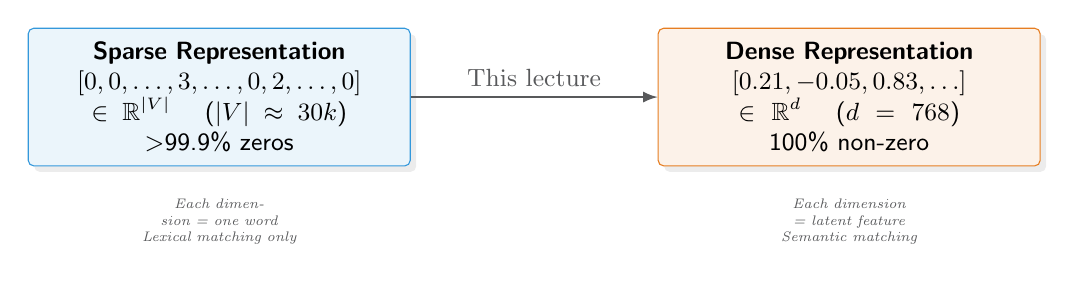
\begin{tikzpicture}
    \node[sparse, text width=4.5cm] (sparse) at (0,0) {\textbf{Sparse Representation}\\
    $[0, 0, \ldots, 3, \ldots, 0, 2, \ldots, 0]$\\
    $\in \mathbb{R}^{|V|}$ \quad ($|V| \approx 30k$)\\
    $>$99.9\% zeros};

    \node[dense, text width=4.5cm] (dense) at (8,0) {\textbf{Dense Representation}\\
    $[0.21, -0.05, 0.83, \ldots]$\\
    $\in \mathbb{R}^{d}$ \quad ($d = 768$)\\
    100\% non-zero};

    \draw[irArrowBase] (sparse) -- (dense) node[midway, above, font=\small, text=irInfra] {This lecture};

    \node[below=0.3cm of sparse, irLabel] {Each dimension = one word\\Lexical matching only};
    \node[below=0.3cm of dense, irLabel] {Each dimension = latent feature\\Semantic matching};
\end{tikzpicture}

\end{center}

\vspace{1em}

\begin{block}{Key Question}
How do we learn dense representations that capture word meaning?
\end{block}
\end{frame}

\begin{frame}{The Distributional Hypothesis}
\begin{block}{Core Principle (Firth, 1957)}
``You shall know a word by the company it keeps.''
\end{block}

\vspace{1em}

\textbf{Example:} What do we know about the word ``\textit{tezguino}''?

\vspace{0.5em}

\begin{itemize}
    \item ``A bottle of \textit{tezguino} is on the table.''
    \item ``Everybody enjoys \textit{tezguino}.''
    \item ``\textit{Tezguino} makes you drunk.''
    \item ``We brew \textit{tezguino} from corn.''
\end{itemize}

\vspace{0.5em}

Without ever seeing a definition, we infer: \textit{tezguino} is an alcoholic beverage.

\vspace{1em}

\begin{exampleblock}{Implication for IR}
Words that appear in similar contexts should have similar vector representations. If we achieve this, ``car'' and ``automobile'' will be close in vector space.
\end{exampleblock}
\end{frame}

\begin{frame}{Word2Vec: Words as Vectors}
\begin{block}{Key Idea (Mikolov et al., 2013)}
Train a neural network to predict context words from a target word (Skip-gram) or a target word from context (CBOW). The learned weight matrix \textit{is} the word embedding.
\end{block}

\vspace{0.5em}

\begin{center}
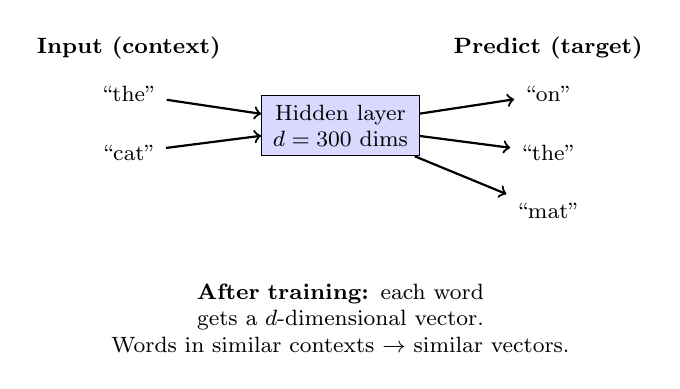
\begin{tikzpicture}[
    node distance=0.8cm,
    box/.style={rectangle, draw, minimum width=2cm, minimum height=0.6cm, font=\footnotesize, align=center},
    arrow/.style={->, thick}
]
    \node[font=\footnotesize] (ctx1) {``the''};
    \node[font=\footnotesize, below=0.3cm of ctx1] (ctx2) {``cat''};
    \node[box, fill=blue!15, right=1.2cm of ctx1, yshift=-0.4cm] (hidden) {Hidden layer\\$d = 300$ dims};
    \node[font=\footnotesize, right=1.2cm of hidden, yshift=0.4cm] (out1) {``on''};
    \node[font=\footnotesize, below=0.3cm of out1] (out2) {``the''};
    \node[font=\footnotesize, below=0.3cm of out2] (out3) {``mat''};

    \draw[arrow] (ctx1) -- (hidden);
    \draw[arrow] (ctx2) -- (hidden);
    \draw[arrow] (hidden) -- (out1);
    \draw[arrow] (hidden) -- (out2);
    \draw[arrow] (hidden) -- (out3);

    \node[above=0.1cm of ctx1, font=\footnotesize\bfseries] {Input (context)};
    \node[above=0.1cm of out1, font=\footnotesize\bfseries] {Predict (target)};

    \node[below=1.5cm of hidden, font=\footnotesize, text width=7cm, align=center] {
    \textbf{After training:} each word gets a $d$-dimensional vector.\\
    Words in similar contexts $\to$ similar vectors.};
\end{tikzpicture}

\end{center}
\end{frame}

\begin{frame}{Word2Vec: Famous Properties}
\begin{block}{Linear Analogies}
$$\vec{\text{king}} - \vec{\text{man}} + \vec{\text{woman}} \approx \vec{\text{queen}}$$
\end{block}

\vspace{0.5em}

\textbf{What this tells us:}
\begin{itemize}
    \item Word vectors capture \textbf{relational structure}
    \item Gender, tense, plurality encoded as directions in vector space
    \item Semantic similarity $\approx$ vector proximity (cosine similarity)
\end{itemize}

\vspace{1em}

\textbf{Relevance to IR:}
\begin{itemize}
    \item $\cos(\vec{\text{car}}, \vec{\text{automobile}}) \approx 0.7$ --- high similarity!
    \item $\cos(\vec{\text{car}}, \vec{\text{banana}}) \approx 0.1$ --- low similarity
    \item Could we use these for retrieval? \textit{Yes, but\ldots}
\end{itemize}

\vspace{0.5em}

\begin{alertblock}{Limitation}
Each word has \textbf{exactly one} vector, regardless of context.\\
``bank'' (river) = ``bank'' (financial) --- same vector!
\end{alertblock}
\end{frame}

\begin{frame}{GloVe: Global Vectors}
\begin{block}{Key Idea (Pennington et al., 2014)}
Instead of predicting context words, directly factorize the \textbf{word co-occurrence matrix}. Objective: $\vec{w}_i \cdot \vec{w}_j$ should approximate $\log(\text{co-occurrence count})$.
\end{block}

\vspace{1em}

\begin{columns}
\begin{column}{0.48\textwidth}
\textbf{Word2Vec vs.\ GloVe:}
\begin{itemize}
    \item Word2Vec: local context windows
    \item GloVe: global co-occurrence statistics
    \item \textbf{In practice:} similar quality
    \item Both produce static, non-contextual vectors
\end{itemize}
\end{column}
\begin{column}{0.48\textwidth}
\textbf{Common dimensions:}
\begin{itemize}
    \item 50d (fast, less accurate)
    \item 100d, 200d (common)
    \item 300d (standard, best quality)
\end{itemize}

\vspace{0.5em}

\textbf{Pre-trained:} Trained on Wikipedia + web data, downloadable.
\end{column}
\end{columns}
\end{frame}

\begin{frame}{From Words to Documents: The Naive Approach}
\begin{block}{Average Word Embeddings}
$$\vec{d} = \frac{1}{|d|}\sum_{w \in d} \vec{w}$$
\end{block}

\vspace{0.5em}

\textbf{Example:} ``the cat sat on the mat''
$$\vec{d} = \frac{\vec{\text{the}} + \vec{\text{cat}} + \vec{\text{sat}} + \vec{\text{on}} + \vec{\text{the}} + \vec{\text{mat}}}{6}$$

\vspace{0.5em}

\begin{columns}
\begin{column}{0.48\textwidth}
\textbf{\textcolor{green}{\checkmark} Advantages:}
\begin{itemize}
    \item Simple and fast
    \item Captures some semantics
    \item Fixed-size output for any doc
\end{itemize}
\end{column}
\begin{column}{0.48\textwidth}
\textbf{\textcolor{red}{\ding{55}} Problems:}
\begin{itemize}
    \item Loses word order completely
    \item ``dog bites man'' = ``man bites dog''
    \item Polysemy unresolved
    \item Rare/important words drowned out
\end{itemize}
\end{column}
\end{columns}

\vspace{0.5em}

\begin{alertblock}{We Need}
Representations where the \textbf{meaning of each word depends on its context}.
\end{alertblock}
\end{frame}

\begin{frame}{Static vs. Contextualized Embeddings}
\begin{center}
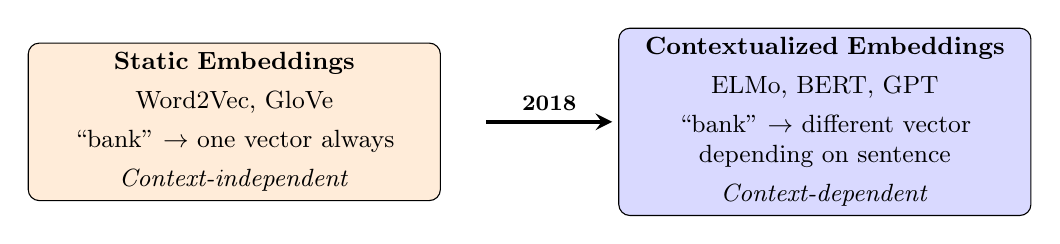
\begin{tikzpicture}[
    box/.style={rectangle, draw, rounded corners, text width=5cm, align=center, minimum height=2cm, font=\small}
]
    \node[box, fill=orange!15] (static) at (0,0) {
        \textbf{Static Embeddings}\\[3pt]
        Word2Vec, GloVe\\[3pt]
        ``bank'' $\to$ one vector always\\[3pt]
        \textit{Context-independent}
    };

    \node[box, fill=blue!15] (context) at (7.5,0) {
        \textbf{Contextualized Embeddings}\\[3pt]
        ELMo, BERT, GPT\\[3pt]
        ``bank'' $\to$ different vector\\depending on sentence\\[3pt]
        \textit{Context-dependent}
    };

    \draw[->, ultra thick, >=stealth] (3.2,0) -- (4.8,0) node[midway, above, font=\footnotesize\bfseries] {2018};
\end{tikzpicture}

\end{center}

\vspace{1em}

\textbf{Example:}
\begin{itemize}
    \item ``I deposited money at the \textbf{bank}.'' $\to$ $\vec{v}_{\text{bank}}^{(1)}$ (financial)
    \item ``We had a picnic by the river \textbf{bank}.'' $\to$ $\vec{v}_{\text{bank}}^{(2)}$ (riverside)
    \item $\vec{v}_{\text{bank}}^{(1)} \neq \vec{v}_{\text{bank}}^{(2)}$ --- polysemy resolved!
\end{itemize}

\vspace{0.5em}

\begin{exampleblock}{Key Insight}
Contextualized embeddings solve both synonymy \textit{and} polysemy.
\end{exampleblock}
\end{frame}

% ====================================================================
% SECTION 2: TRANSFORMERS & ATTENTION
% ====================================================================
\section{The Transformer Architecture}

\begin{frame}[plain]
\sectionpage
\end{frame}

\begin{frame}{Why Transformers?}
\begin{block}{Before Transformers (pre-2017)}
Sequential models (RNNs, LSTMs):
\begin{itemize}
    \item Process words one at a time, left to right
    \item Long-range dependencies are hard (vanishing gradients)
    \item Cannot parallelize training (each step depends on previous)
\end{itemize}
\end{block}

\vspace{1em}

\begin{block}{The Transformer Insight (Vaswani et al., 2017)}
\textbf{``Attention Is All You Need''}
\begin{itemize}
    \item Process all words \textbf{simultaneously} (parallel)
    \item Each word attends to \textbf{every other word} directly
    \item No sequential bottleneck $\to$ massively faster training
    \item Result: the foundation of BERT, GPT, and all modern NLP
\end{itemize}
\end{block}
\end{frame}

\begin{frame}{Encoder Model Architecture}
\begin{center}
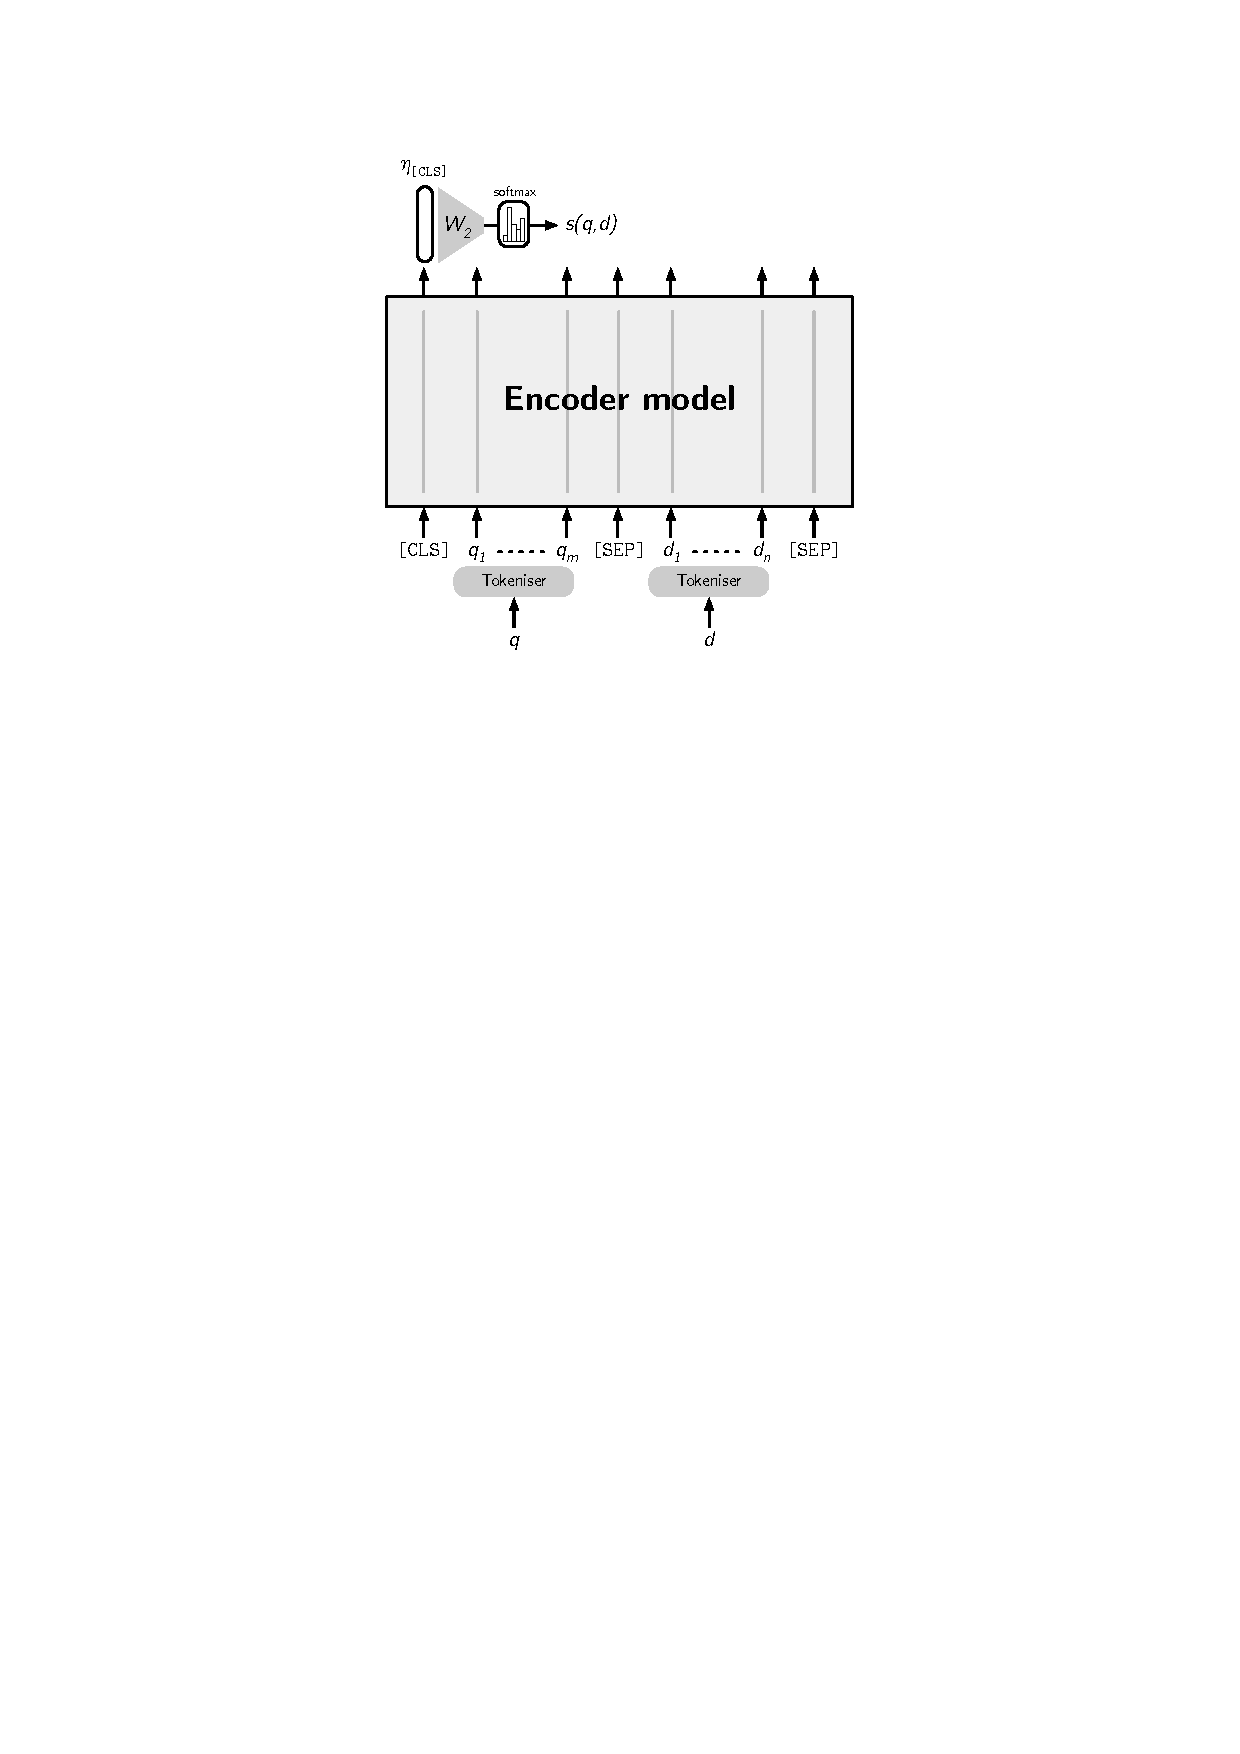
\includegraphics[width=0.75\textwidth]{figures/embeddings-encoder-model.pdf}
\end{center}
\end{frame}


\begin{frame}{Self-Attention: The Core Mechanism}
\begin{block}{Intuition}
For each word in the input, self-attention asks: ``Which other words should I pay attention to in order to understand the meaning of \textit{this} word?''
\end{block}

\vspace{0.5em}

\textbf{Example:} ``The animal didn't cross the street because \textbf{it} was too tired.''

\vspace{0.3em}

What does ``it'' refer to? \textbf{The animal.}

\vspace{0.3em}

Self-attention learns to connect ``it'' $\to$ ``animal'' by assigning a high attention weight between them.

\vspace{1em}

\begin{center}
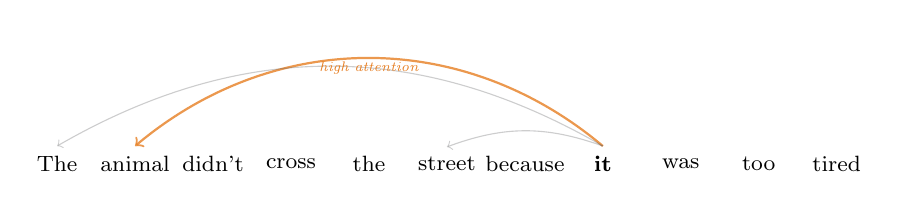
\begin{tikzpicture}[scale=0.9]
    \foreach \i/\word in {0/The, 1/animal, 2/didn't, 3/cross, 4/the, 5/street, 6/because, 7/\textbf{it}, 8/was, 9/too, 10/tired} {
        \node[font=\footnotesize] (w\i) at (\i*1.1, 0) {\word};
    }
    \draw[->, thick, irDense, opacity=0.8] (w7.north) to[bend right=40] (w1.north);
    \draw[->, thin, irInfra, opacity=0.3] (w7.north) to[bend right=30] (w0.north);
    \draw[->, thin, irInfra, opacity=0.3] (w7.north) to[bend right=20] (w5.north);
    \node[above=0.8cm of w4, irLabel, text=irDense] {high attention};
\end{tikzpicture}

\end{center}
\end{frame}

\begin{frame}{Self-Attention: Query, Key, Value}
\begin{block}{Formal Mechanism}
Each word $w_i$ is projected into three vectors:
\begin{itemize}
    \item \textbf{Query} $\vec{q}_i$: ``What am I looking for?''
    \item \textbf{Key} $\vec{k}_i$: ``What do I contain?''
    \item \textbf{Value} $\vec{v}_i$: ``What information do I provide?''
\end{itemize}
\end{block}

\vspace{0.5em}

\textbf{Attention computation:}
$$\text{Attention}(Q, K, V) = \text{softmax}\left(\frac{QK^T}{\sqrt{d_k}}\right) V$$

\vspace{0.5em}

\textbf{Step by step:}
\begin{enumerate}
    \item Compute similarity: $\vec{q}_i \cdot \vec{k}_j$ for all pairs $(i, j)$
    \item Scale by $\sqrt{d_k}$ to prevent extreme values
    \item Softmax $\to$ attention weights (sum to 1)
    \item Weighted sum of value vectors $\to$ new representation for word $i$
\end{enumerate}

\vspace{0.5em}

\begin{exampleblock}{Key Point}
Every word's output is a \textbf{weighted combination of all words' values}, where weights are learned based on content similarity.
\end{exampleblock}
\end{frame}

\begin{frame}{Self-Attention: Worked Example (1/2)}
\textbf{Sentence:} ``retrieval models'' (2 tokens for simplicity, $d_k = 2$)

\vspace{0.5em}

\textbf{Projections} (learned weight matrices):
\begin{columns}
\begin{column}{0.5\textwidth}
\begin{align*}
\vec{q}_{\text{retrieval}} &= [1.0, 0.5] \\
\vec{k}_{\text{retrieval}} &= [0.8, 0.2] \\
\vec{v}_{\text{retrieval}} &= [0.3, 0.9]
\end{align*}
\end{column}
\begin{column}{0.5\textwidth}
\begin{align*}
\vec{q}_{\text{models}} &= [0.3, 1.2] \\
\vec{k}_{\text{models}} &= [0.1, 1.0] \\
\vec{v}_{\text{models}} &= [0.7, 0.4]
\end{align*}
\end{column}
\end{columns}

\vspace{1em}

\textbf{Step 1: Dot products} ($\vec{q}_i \cdot \vec{k}_j$):
\begin{align*}
\text{retrieval} \to \text{retrieval}: &\quad 1.0 \times 0.8 + 0.5 \times 0.2 = 0.9 \\
\text{retrieval} \to \text{models}: &\quad 1.0 \times 0.1 + 0.5 \times 1.0 = 0.6
\end{align*}

\vspace{0.5em}

\textbf{Step 2: Scale by $\sqrt{d_k} = \sqrt{2} \approx 1.41$}: \quad $[0.64, 0.43]$
\end{frame}

\begin{frame}{Self-Attention: Worked Example (2/2)}
\textbf{Recall:} Computing attention for ``retrieval'' in ``retrieval models''

\vspace{0.5em}

\textbf{After scaling:} $[0.64, 0.43]$

\vspace{1em}

\textbf{Step 3: Softmax} (normalize to probabilities):
$$\text{softmax}([0.64, 0.43]) = [\,0.55,\; 0.45\,]$$

These are the \textbf{attention weights}: how much ``retrieval'' attends to each token.

\vspace{1em}

\textbf{Step 4: Weighted sum of values}:
\begin{align*}
\vec{h}_{\text{retrieval}} &= 0.55 \times \vec{v}_{\text{retrieval}} + 0.45 \times \vec{v}_{\text{models}} \\
&= 0.55 \times [0.3, 0.9] + 0.45 \times [0.7, 0.4] \\
&= [0.48, 0.68]
\end{align*}

\vspace{0.5em}

\begin{exampleblock}{Result}
The output for ``retrieval'' now incorporates information from ``models''!
\end{exampleblock}
\end{frame}

\begin{frame}[shrink=5]{Multi-Head Attention}
\begin{block}{Problem}
A single attention head can only capture one type of relationship. But words relate to each other in multiple ways (syntactic, semantic, positional).
\end{block}

\vspace{0.5em}

\begin{block}{Solution: Multiple Heads}
Run $h$ separate attention computations in parallel, each with its own $Q$, $K$, $V$ projections. Concatenate and project:
$$\text{MultiHead}(Q, K, V) = \text{Concat}(\text{head}_1, \ldots, \text{head}_h) \cdot W^O$$
\end{block}

\vspace{0.5em}

\textbf{BERT uses $h = 12$ heads.} Each head can learn different patterns:
\begin{itemize}
    \item Head 1: subject-verb relationships
    \item Head 2: adjective-noun relationships
    \item Head 3: coreference (``it'' $\to$ ``animal'')
    \item Head 4: positional/sequential patterns
\end{itemize}
\end{frame}

\begin{frame}[shrink=5]{Positional Encoding}
\begin{alertblock}{Problem}
Self-attention is permutation-invariant --- ``dog bites man'' and ``man bites dog'' produce the same attention weights! Word order is lost.
\end{alertblock}

\vspace{1em}

\begin{block}{Solution: Add Position Information}
Before feeding tokens to the transformer, add a \textbf{positional encoding} vector to each word embedding:
$$\vec{x}_i = \vec{e}_{\text{word}_i} + \vec{p}_i$$
\end{block}

\vspace{0.5em}

\textbf{Sinusoidal encoding} (Vaswani et al.):
\begin{align*}
PE_{(pos, 2i)} &= \sin(pos / 10000^{2i/d}) \\
PE_{(pos, 2i+1)} &= \cos(pos / 10000^{2i/d})
\end{align*}

Each position gets a unique pattern. Nearby positions have similar encodings.

\vspace{0.5em}

\textit{BERT uses learned positional embeddings instead (up to 512 positions).}
\end{frame}

\begin{frame}{The Transformer Encoder Block}
\begin{center}
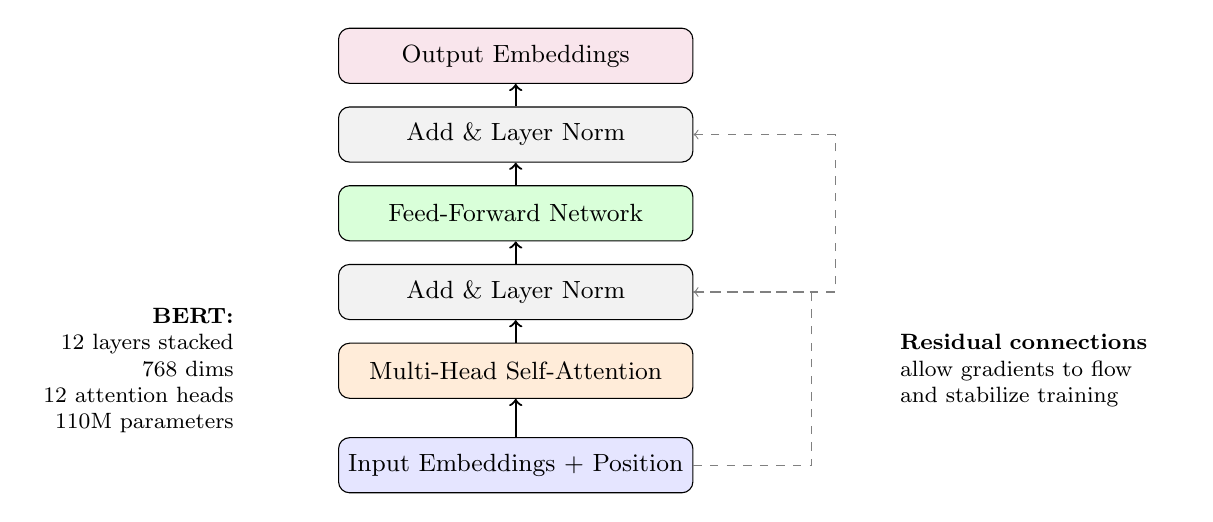
\begin{tikzpicture}[
    block/.style={rectangle, draw, rounded corners, minimum width=4.5cm, minimum height=0.7cm, align=center, font=\small},
    arrow/.style={->, thick}
]
    \node[block, fill=blue!10] (input) at (0, 0) {Input Embeddings + Position};
    \node[block, fill=orange!15] (attn) at (0, 1.2) {Multi-Head Self-Attention};
    \node[block, fill=gray!10] (add1) at (0, 2.2) {Add \& Layer Norm};
    \node[block, fill=green!15] (ffn) at (0, 3.2) {Feed-Forward Network};
    \node[block, fill=gray!10] (add2) at (0, 4.2) {Add \& Layer Norm};
    \node[block, fill=purple!10] (out) at (0, 5.2) {Output Embeddings};

    \draw[arrow] (input) -- (attn);
    \draw[arrow] (attn) -- (add1);
    \draw[arrow] (add1) -- (ffn);
    \draw[arrow] (ffn) -- (add2);
    \draw[arrow] (add2) -- (out);

    % Residual connections
    \draw[->, dashed, gray] (input.east) -- ++(1.5,0) |- (add1.east);
    \draw[->, dashed, gray] (add1.east) -- ++(1.8,0) |- (add2.east);

    \node[right=2.5cm of attn, text width=3.5cm, font=\footnotesize] {
        \textbf{Residual connections}\\
        allow gradients to flow\\
        and stabilize training
    };

    \node[left=1.2cm of attn, font=\footnotesize, text width=2.5cm, align=right] {
        \textbf{BERT:}\\
        12 layers stacked\\
        768 dims\\
        12 attention heads\\
        110M parameters
    };
\end{tikzpicture}

\end{center}
\end{frame}


% ====================================================================
% SECTION 3: BERT FOR IR
% ====================================================================
\section{BERT for Information Retrieval}

\begin{frame}[plain]
\sectionpage
\end{frame}

\begin{frame}{BERT: Pre-training}
\begin{block}{Bidirectional Encoder Representations from Transformers (Devlin et al., 2019)}
A transformer encoder pre-trained on massive text with two objectives:
\end{block}

\vspace{0.5em}

\begin{columns}
\begin{column}{0.48\textwidth}
\textbf{1. Masked Language Modeling (MLM)}
\begin{itemize}
    \item Randomly mask 15\% of tokens
    \item Predict masked tokens from context
    \item Bidirectional (sees left \textit{and} right)
\end{itemize}

\vspace{0.3em}

\textbf{Input:} ``The [MASK] sat on the mat''\\
\textbf{Predict:} ``cat'' (from context)
\end{column}

\begin{column}{0.48\textwidth}
\textbf{2. Next Sentence Prediction (NSP)}
\begin{itemize}
    \item Given sentence A, is sentence B the actual next sentence?
    \item Binary classification
    \item Learns inter-sentence relationships
\end{itemize}

\vspace{0.3em}

\textbf{A:} ``The cat sat on the mat.''\\
\textbf{B:} ``It was very comfortable.'' \checkmark
\end{column}
\end{columns}

\vspace{1em}

\begin{exampleblock}{Pre-training Data}
BooksCorpus (800M words) + English Wikipedia (2.5B words). Trained for 4 days on 16 TPUs.
\end{exampleblock}
\end{frame}

\begin{frame}{BERT: Why It Matters for IR (1/2)}
\begin{block}{Key Properties}
\begin{enumerate}
    \item \textbf{Bidirectional context:} Every token sees all other tokens (not just left-to-right like GPT)
    \item \textbf{Deep:} 12 layers of attention $\to$ rich, hierarchical representations
    \item \textbf{Pre-trained:} Learned from billions of words $\to$ knows language
    \item \textbf{Fine-tunable:} Adapt to specific tasks with small labeled data
\end{enumerate}
\end{block}

\vspace{1em}

\begin{exampleblock}{Transfer Learning}
BERT brings the power of transfer learning to NLP: pre-train once on massive data, fine-tune for specific tasks with minimal labeled data.
\end{exampleblock}
\end{frame}

\begin{frame}{BERT: Why It Matters for IR (2/2)}
\textbf{For IR, BERT can:}
\begin{itemize}
    \item Understand that ``automobile issues'' is related to ``car problems''
    \item Disambiguate ``bank'' based on surrounding context
    \item Capture negation: ``not relevant'' $\neq$ ``relevant''
    \item Handle word order: ``python eats mouse'' $\neq$ ``mouse eats python''
\end{itemize}

\vspace{1em}

\begin{alertblock}{Recall}
None of this was possible with BM25 or static embeddings.
\end{alertblock}
\end{frame}

\begin{frame}{Cross-Encoder: BERT for Re-ranking}
\begin{block}{Architecture (Nogueira \& Cho, 2019)}
Feed the query and document \textbf{together} through BERT. Use the \texttt{[CLS]} token output as a relevance score.
\end{block}

\vspace{0.5em}

\begin{center}
\begin{tikzpicture}[scale=0.8, transform shape]
    % Input tokens (generic style)
    \node[muted, compact] (cls) at (0, 0) {[CLS]};
    \node[rerank, compact, fill=irRerank!10] (q1) at (1.1, 0) {car};
    \node[rerank, compact, fill=irRerank!10] (q2) at (2.2, 0) {problems};
    \node[muted, compact] (sep1) at (3.3, 0) {[SEP]};
    \node[rerank, compact, fill=irHybrid!10, draw=irHybrid] (d1) at (4.4, 0) {auto};
    \node[rerank, compact, fill=irHybrid!10, draw=irHybrid] (d2) at (5.5, 0) {\#\#mobile};
    \node[rerank, compact, fill=irHybrid!10, draw=irHybrid] (d3) at (6.6, 0) {issues};
    \node[rerank, compact, fill=irHybrid!10, draw=irHybrid] (d4) at (7.7, 0) {and};
    \node[rerank, compact, fill=irHybrid!10, draw=irHybrid] (d5) at (8.8, 0) {fixes};
    \node[muted, compact] (sep2) at (9.9, 0) {[SEP]};

    % BERT block
    \node[rerank, minimum width=9.9cm, minimum height=1.5cm, fill=irRerank!20, thick] (bert) at (4.95, 2.2) {\textbf{BERT} (12 layers $\times$ 12 heads)\\Full cross-attention between \textcolor{irRerank}{query} and \textcolor{irHybrid}{document}};
    % Output
    \node[rerank, minimum width=1.5cm, fill=irRerank!30] (clsout) at (0, 4.5) {$h_{\text{[CLS]}}$};
    \node[rerank, minimum width=2.5cm, fill=irRerank!40] (score) at (0, 6.2) {$P(\text{rel}) = \sigma(W \cdot h_{\text{[CLS]}})$};

    % Arrows
    \foreach \n in {cls, q1, q2, sep1, d1, d2, d3, d4, d5, sep2} {
        \draw[irArrowBase, thin] (\n.north) -- (\n.north |- bert.south);
    }
    \draw[irArrowBase] (bert.north -| clsout) -- (clsout.south);
    \draw[irArrowBase] (clsout) -- (score);

    % Labels
    \node[left=0.1cm of cls, font=\tiny\bfseries\color{irRerank}] {Query};
    \node[left=0.1cm of d1, font=\tiny\bfseries\color{irHybrid}] {Document};
\end{tikzpicture}

\end{center}
\end{frame}

\begin{frame}{Cross-Encoder Architecture (Detailed)}
\begin{center}
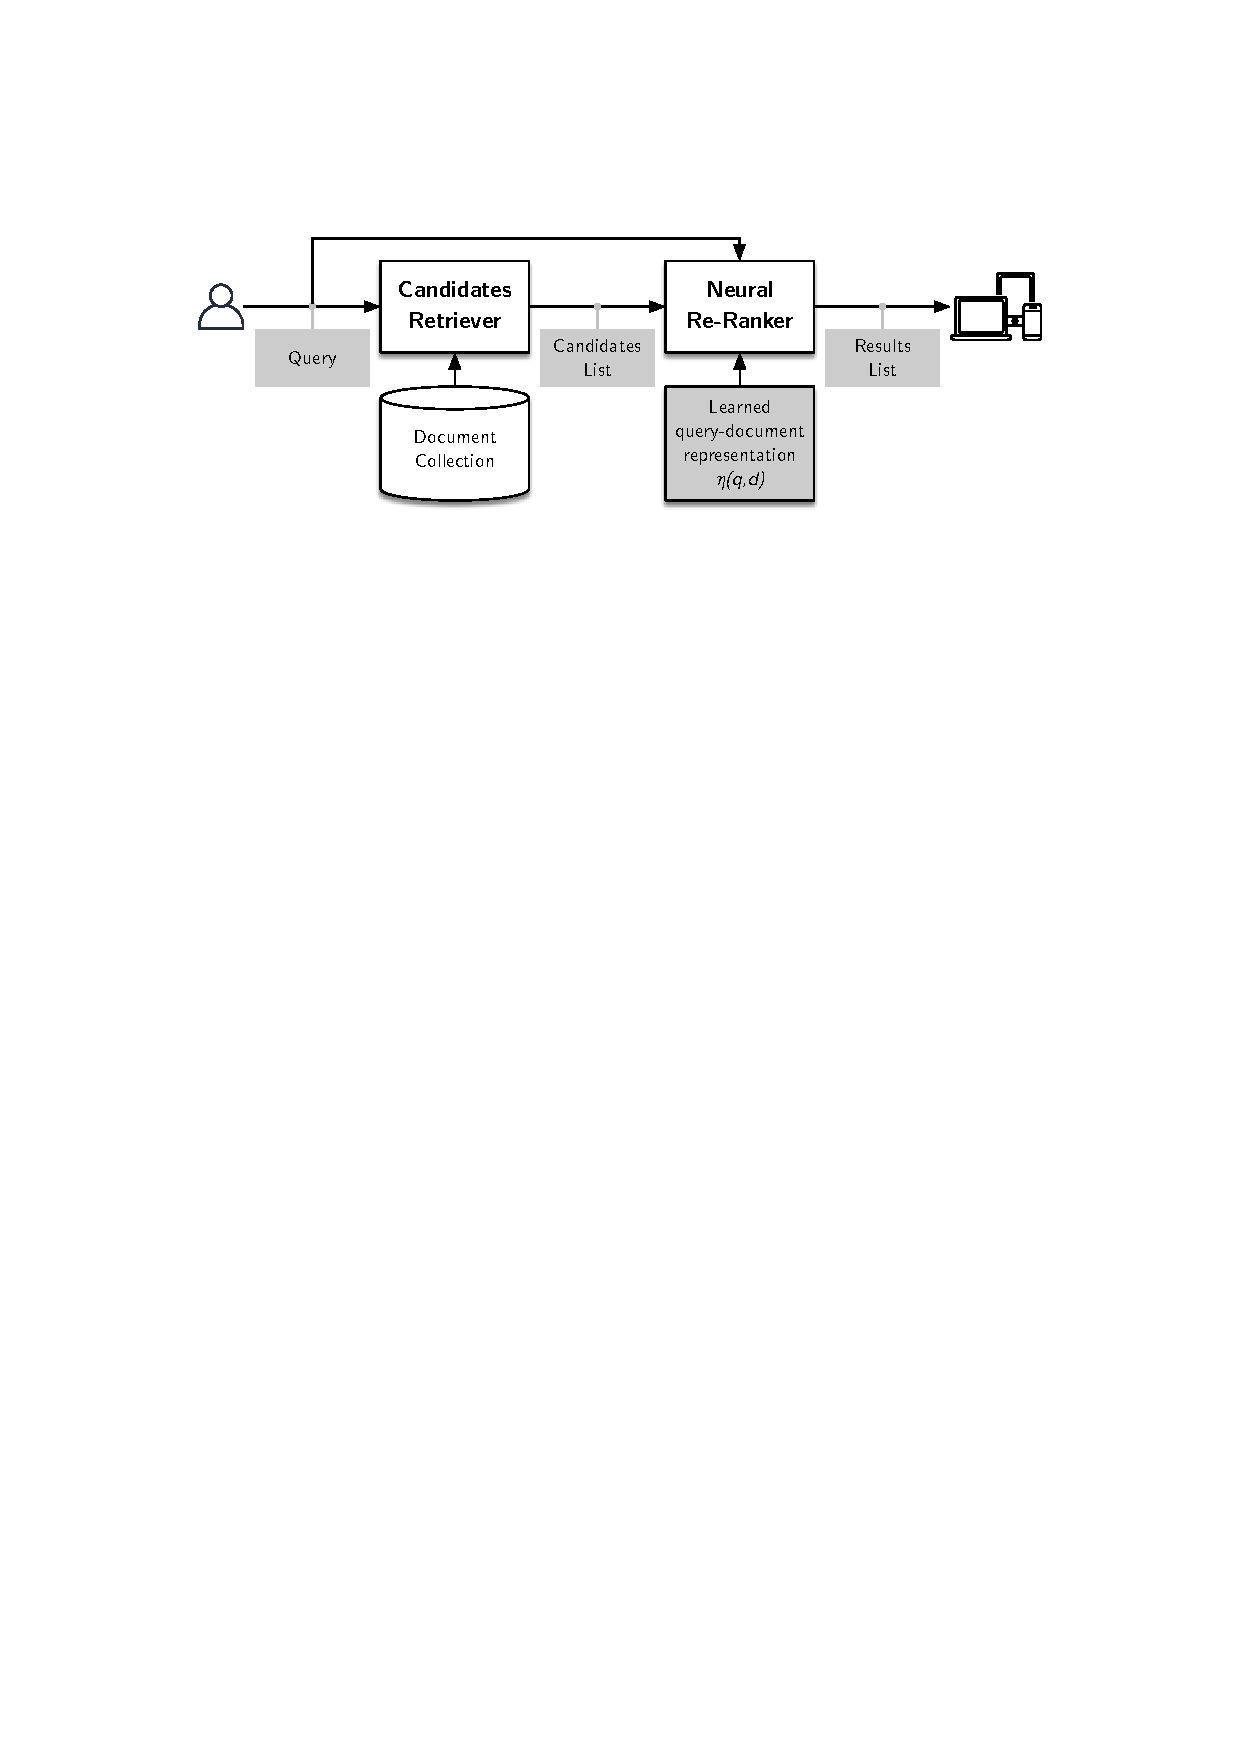
\includegraphics[width=0.85\textwidth]{figures/cross-encoder-ranking.pdf}
\end{center}
\end{frame}


\begin{frame}{Cross-Encoder: Why It Works}
\begin{block}{Full Cross-Attention}
Every query token attends to every document token (and vice versa) through all 12 layers. This enables:
\end{block}

\vspace{0.5em}

\begin{enumerate}
    \item \textbf{Soft matching:} ``car'' attends to ``automobile'' $\to$ learns they're related
    \item \textbf{Context understanding:} ``not working'' is different from ``working''
    \item \textbf{Relevance patterns:} The model learns what makes a document relevant to a query, not just topical overlap
\end{enumerate}

\vspace{1em}

\begin{columns}
\begin{column}{0.48\textwidth}
\textbf{\textcolor{green}{\checkmark} Strengths:}
\begin{itemize}
    \item Most accurate neural ranking
    \item Rich query-document interaction
    \item Pre-trained knowledge
\end{itemize}
\end{column}
\begin{column}{0.48\textwidth}
\textbf{\textcolor{red}{\ding{55}} Limitations:}
\begin{itemize}
    \item Must encode \textit{every} (q, d) pair
    \item Cannot pre-compute doc embeddings
    \item Too slow for full-corpus retrieval
\end{itemize}
\end{column}
\end{columns}
\end{frame}

\begin{frame}{Cross-Encoder: Latency Analysis}
\textbf{How slow is ``too slow''?}

\vspace{1em}

\begin{table}
\centering
\begin{tabular}{lccl}
\toprule
\textbf{Candidates} & \textbf{Time/pair} & \textbf{Total} & \textbf{Feasible?} \\
\midrule
1{,}000{,}000 (full corpus) & 5 ms & 5{,}000 s & \textcolor{red}{\ding{55} No} \\
10{,}000 & 5 ms & 50 s & \textcolor{red}{\ding{55} No} \\
1{,}000 & 5 ms & 5 s & \textcolor{orange}{Borderline} \\
\textbf{100} & \textbf{5 ms} & \textbf{0.5 s} & \textcolor{green}{\checkmark Yes} \\
20 & 5 ms & 0.1 s & \textcolor{green}{\checkmark Yes} \\
\bottomrule
\end{tabular}
\end{table}

\vspace{1em}

\begin{exampleblock}{Conclusion}
Cross-encoders can realistically re-rank the \textbf{top 100--1000} documents from a first-stage retriever. They \textbf{cannot} replace the retriever itself.
\end{exampleblock}

\vspace{0.5em}

This is why we need \textbf{the two-stage pipeline}.
\end{frame}

\begin{frame}{Worked Example: Cross-Encoder Scoring (1/2)}
\textbf{Query:} ``side effects of aspirin''

\vspace{1em}

\textbf{Doc A:} ``Aspirin may cause stomach bleeding and ringing in the ears as common adverse reactions.''

\vspace{0.5em}

\textbf{Doc B:} ``The company's stock price went up after the aspirin sales report.''

\vspace{1em}

\textbf{Step 1: Tokenization} (WordPiece):
{\small
\begin{itemize}
    \item \texttt{[CLS] side effects of aspirin [SEP] aspirin may cause stomach bleeding and ringing in the ears as common adverse reactions . [SEP]}
    \item \texttt{[CLS] side effects of aspirin [SEP] the company ' s stock price went up after the aspirin sales report . [SEP]}
\end{itemize}
}

\vspace{0.5em}

\textbf{Step 2: BERT processes each pair} (full cross-attention between query and document tokens)
\end{frame}

\begin{frame}{Worked Example: Cross-Encoder Scoring (2/2)}
\textbf{Query:} ``side effects of aspirin''

\vspace{0.5em}

\textbf{Step 3: Classification head on [CLS]}:
\begin{itemize}
    \item \textbf{Doc A:} ``adverse reactions'', ``bleeding'', ``stomach'' $\to$ high attention to ``side effects''
    \begin{itemize}
        \item $P(\text{rel}) = \mathbf{0.94}$ \textcolor{green}{\checkmark}
    \end{itemize}

    \vspace{0.5em}

    \item \textbf{Doc B:} ``stock price'', ``sales report'' $\to$ low attention to ``side effects''
    \begin{itemize}
        \item $P(\text{rel}) = \mathbf{0.12}$ \textcolor{red}{\ding{55}}
    \end{itemize}
\end{itemize}

\vspace{1em}

\begin{exampleblock}{Why This Works}
BM25 might rank Doc B highly too (it contains ``aspirin''). The cross-encoder understands that the \textit{topic} doesn't match the query intent.
\end{exampleblock}
\end{frame}

\begin{frame}{Fine-Tuning BERT for Ranking (1/2)}
\begin{block}{Training Data}
Pairs of (query, document) with relevance labels:
\begin{itemize}
    \item \textbf{MS MARCO:} 530K queries with sparse judgments (1 relevant passage per query)
    \item \textbf{TREC:} Dense judgments (multiple levels: 0, 1, 2, 3)
\end{itemize}
\end{block}

\vspace{1em}

\textbf{Training objective:}
\begin{itemize}
    \item \textbf{Pointwise:} Binary cross-entropy on $P(\text{rel})$ for each (q, d)
    \begin{itemize}
        \item Simpler, treats each pair independently
    \end{itemize}

    \vspace{0.5em}

    \item \textbf{Pairwise:} Given $(q, d^+, d^-)$, train so $\text{score}(q, d^+) > \text{score}(q, d^-)$
    \begin{itemize}
        \item Better ranking performance
    \end{itemize}
\end{itemize}
\end{frame}

\begin{frame}{Fine-Tuning BERT for Ranking (2/2)}
\textbf{Practical fine-tuning setup:}
\begin{itemize}
    \item Start from pre-trained BERT checkpoint (e.g., \texttt{bert-base-uncased})
    \item Fine-tune on IR data for 2--3 epochs
    \item Learning rate: $2 \times 10^{-5}$ (small, to preserve pre-trained knowledge)
    \item Max sequence length: 512 tokens
    \begin{itemize}
        \item Query $\approx$ 10 tokens + Document $\approx$ 500 tokens
    \end{itemize}
\end{itemize}

\vspace{1em}

\begin{exampleblock}{Training Time}
Fine-tuning BERT-base on MS MARCO: $\sim$12--24 hours on a single GPU.
\end{exampleblock}

\vspace{0.5em}

\begin{alertblock}{Key Point}
We're \textbf{fine-tuning}, not training from scratch. This leverages BERT's pre-trained language understanding.
\end{alertblock}
\end{frame}

\begin{frame}{monoBERT and monoT5}
\begin{columns}
\begin{column}{0.48\textwidth}
\begin{block}{monoBERT}
\begin{itemize}
    \item BERT-base or BERT-large
    \item Classification head on [CLS]
    \item Input: [CLS] q [SEP] d [SEP]
    \item Output: $P(\text{relevant})$
    \item \textbf{110M--340M parameters}
\end{itemize}

\vspace{0.3em}

Nogueira \& Cho (2019)
\end{block}
\end{column}

\begin{column}{0.48\textwidth}
\begin{block}{monoT5}
\begin{itemize}
    \item T5 (encoder-decoder)
    \item Input: ``Query: q Document: d Relevant:''
    \item Output: ``true'' or ``false''
    \item Score = $P(\text{``true''})$
    \item \textbf{220M--3B parameters}
\end{itemize}

\vspace{0.3em}

Nogueira et al.\ (2020)
\end{block}
\end{column}
\end{columns}

\vspace{1em}

\begin{exampleblock}{Comparison}
\begin{itemize}
    \item monoT5 (3B) slightly outperforms monoBERT on most benchmarks
    \item Both are cross-encoders (same speed limitation)
    \item monoBERT more popular due to simplicity and availability
\end{itemize}
\end{exampleblock}
\end{frame}

\begin{frame}{ColBERT: Late Interaction (Preview)}
\begin{block}{Key Idea (Khattab \& Zaharia, 2020)}
A middle ground between cross-encoders and bi-encoders: encode query and document \textbf{separately}, but compare at the \textbf{token level} using MaxSim.
\end{block}

\vspace{0.5em}

\begin{center}
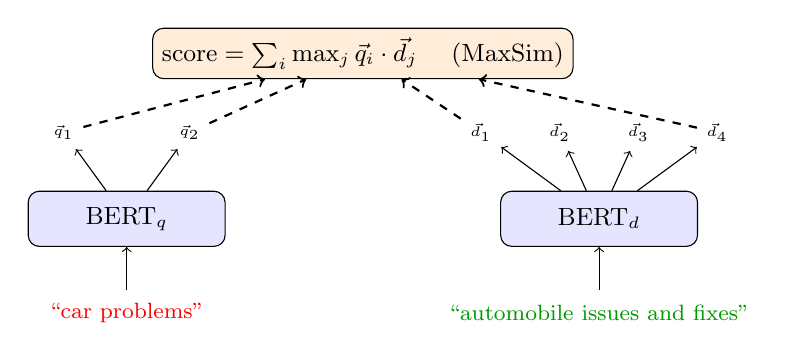
\begin{tikzpicture}[
    box/.style={rectangle, draw, rounded corners, fill=blue!10, minimum height=0.7cm, align=center, font=\small},
    arrow/.style={->, thick}
]
    \node[box, minimum width=2.5cm] (bq) at (0, 1.5) {BERT$_q$};
    \node[box, minimum width=2.5cm] (bd) at (6, 1.5) {BERT$_d$};

    \node[font=\footnotesize, red] at (0, 0.3) {``car problems''};
    \node[font=\footnotesize, green!60!black] at (6, 0.3) {``automobile issues and fixes''};

    \node[font=\tiny] (e1) at (-0.8, 2.6) {$\vec{q}_1$};
    \node[font=\tiny] (e2) at (0.8, 2.6) {$\vec{q}_2$};

    \node[font=\tiny] (d1) at (4.5, 2.6) {$\vec{d}_1$};
    \node[font=\tiny] (d2) at (5.5, 2.6) {$\vec{d}_2$};
    \node[font=\tiny] (d3) at (6.5, 2.6) {$\vec{d}_3$};
    \node[font=\tiny] (d4) at (7.5, 2.6) {$\vec{d}_4$};

    \draw[arrow, thin] (0, 0.6) -- (bq);
    \draw[arrow, thin] (6, 0.6) -- (bd);

    \draw[arrow, thin] (bq) -- (e1);
    \draw[arrow, thin] (bq) -- (e2);
    \draw[arrow, thin] (bd) -- (d1);
    \draw[arrow, thin] (bd) -- (d2);
    \draw[arrow, thin] (bd) -- (d3);
    \draw[arrow, thin] (bd) -- (d4);

    \node[rectangle, draw, fill=orange!15, rounded corners, font=\small] (maxsim) at (3, 3.6) {$\text{score} = \sum_i \max_j \vec{q}_i \cdot \vec{d}_j$ \quad (MaxSim)};

    \draw[arrow, dashed] (e1) -- (maxsim);
    \draw[arrow, dashed] (e2) -- (maxsim);
    \draw[arrow, dashed] (d1) -- (maxsim);
    \draw[arrow, dashed] (d4) -- (maxsim);
\end{tikzpicture}

\end{center}
\end{frame}

\begin{frame}{ColBERT: Why It Matters}
\begin{block}{MaxSim Scoring}
For each query token $q_i$, find the document token $d_j$ with highest cosine similarity. Sum across all query tokens:
$$\text{score}(q, d) = \sum_{i=1}^{|q|} \max_{j=1}^{|d|}\; \vec{q}_i \cdot \vec{d}_j$$
\end{block}

\vspace{0.5em}

\begin{table}
\centering
\footnotesize
\begin{tabular}{lccc}
\toprule
& \textbf{Cross-Encoder} & \textbf{ColBERT} & \textbf{Bi-Encoder} \\
\midrule
Interaction & Full (all layers) & Late (token-level) & None (single vector) \\
Pre-compute docs & \textcolor{red}{\ding{55}} No & \textcolor{green}{\checkmark} Yes (per-token) & \textcolor{green}{\checkmark} Yes (single vec) \\
Use for retrieval & \textcolor{red}{\ding{55}} No & \textcolor{green}{\checkmark} With ANN & \textcolor{green}{\checkmark} With ANN \\
Accuracy & Highest & Near cross-encoder & Lower \\
Storage per doc & N/A & $|d| \times 128$ floats & $1 \times 768$ floats \\
\bottomrule
\end{tabular}
\end{table}

\vspace{0.5em}

\begin{exampleblock}{Takeaway}
ColBERT gives near-cross-encoder accuracy with bi-encoder-like speed. Trade-off: \textbf{much higher storage} (one vector per token, not per document). We'll revisit ColBERT in detail in Lecture 5.
\end{exampleblock}
\end{frame}

% ====================================================================
% NEW SECTION: TRAINING CROSS-ENCODERS
% ====================================================================
\section{Training Cross-Encoders in Practice}

\begin{frame}[plain]
\sectionpage
\end{frame}

\begin{frame}{MS MARCO: The Standard Training Dataset}
\begin{block}{MS MARCO Passage Ranking (Nguyen et al., 2016)}
\begin{itemize}
    \item \textbf{8.8M passages} from web documents
    \item \textbf{530K training queries} with sparse relevance labels
    \item Each query has $\sim$1 relevant passage (sometimes 2--3)
    \item \textbf{6,980 dev queries} for validation
\end{itemize}
\end{block}

\vspace{1em}

\begin{exampleblock}{Scale}
This is the largest publicly available passage ranking dataset, widely used for training neural rankers.
\end{exampleblock}
\end{frame}

\begin{frame}{MS MARCO: The Sparse Labels Challenge}
\begin{alertblock}{Key Challenge: Sparse Labels}
For each query, only $\sim$1 passage is labeled relevant out of 8.8M. That means:
\begin{itemize}
    \item Many relevant passages are \textbf{unlabeled} (false negatives)
    \item We can't treat all unlabeled passages as truly non-relevant
    \item Negative sampling strategy matters enormously
\end{itemize}
\end{alertblock}

\vspace{1em}

\textbf{Implication for training:}
\begin{itemize}
    \item Random negatives are too easy
    \item Need \textbf{hard negatives} from BM25 top-$k$
    \item This forces the model to learn beyond lexical matching
\end{itemize}
\end{frame}

\begin{frame}[shrink=5]{Training Pipeline: Step by Step}
\begin{center}
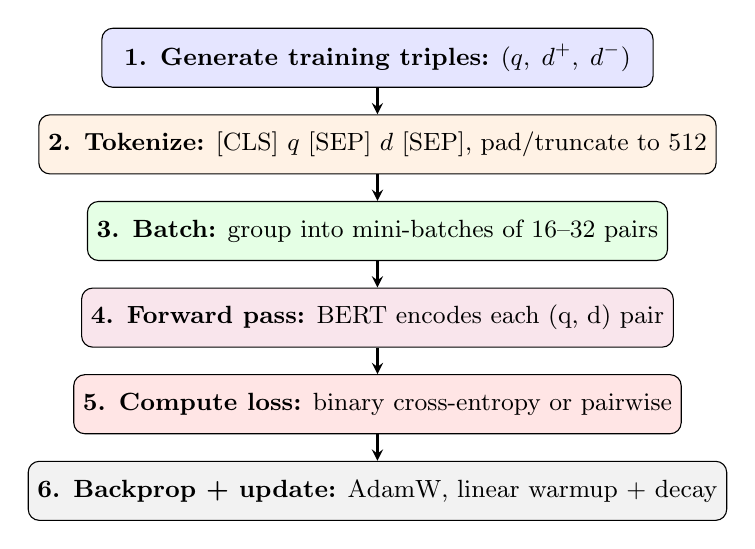
\begin{tikzpicture}[
    node distance=1.1cm,
    box/.style={rectangle, draw, rounded corners, minimum width=7cm, minimum height=0.75cm, align=center, font=\small},
    arrow/.style={->, thick, >=stealth}
]
    \node[box, fill=blue!10] (triples) {\textbf{1. Generate training triples:} $(q,\; d^+,\; d^-)$};
    \node[box, fill=orange!10, below of=triples] (tokenize) {\textbf{2. Tokenize:} [CLS] $q$ [SEP] $d$ [SEP], pad/truncate to 512};
    \node[box, fill=green!10, below of=tokenize] (batch) {\textbf{3. Batch:} group into mini-batches of 16--32 pairs};
    \node[box, fill=purple!10, below of=batch] (forward) {\textbf{4. Forward pass:} BERT encodes each (q, d) pair};
    \node[box, fill=red!10, below of=forward] (loss) {\textbf{5. Compute loss:} binary cross-entropy or pairwise};
    \node[box, fill=gray!10, below of=loss] (update) {\textbf{6. Backprop + update:} AdamW, linear warmup + decay};

    \draw[arrow] (triples) -- (tokenize);
    \draw[arrow] (tokenize) -- (batch);
    \draw[arrow] (batch) -- (forward);
    \draw[arrow] (forward) -- (loss);
    \draw[arrow] (loss) -- (update);
\end{tikzpicture}

\end{center}

\vspace{0.5em}

\textbf{Typical training:} 2--3 epochs over MS MARCO triples, $\sim$12--24 hours on a single GPU.
\end{frame}

\begin{frame}{Negative Sampling Strategies}
\begin{block}{The Core Question}
Query has 1 labeled positive. Where do the negatives come from?
\end{block}

\vspace{1em}

\begin{enumerate}
    \item \textbf{Random negatives}
    \begin{itemize}
        \item Sample random passage from corpus
        \item Easy for model to distinguish $\to$ weak training signal
        \item \textcolor{red}{\ding{55}} Not recommended for production
    \end{itemize}

    \vspace{0.5em}

    \item \textbf{BM25 hard negatives} \textcolor{green}{\checkmark} \textit{Recommended}
    \begin{itemize}
        \item Run BM25, take top-$k$ \textit{non-relevant} passages
        \item These are topically related but not relevant $\to$ strong signal
        \item Forces model to learn beyond term overlap
    \end{itemize}
\end{enumerate}
\end{frame}

\begin{frame}{Training Hyperparameters}
\begin{columns}
\begin{column}{0.48\textwidth}
\textbf{Batching \& Memory}
\begin{itemize}
    \item Max seq length 512 tokens
    \item Batch size 16--32 (limited by GPU)
    \item \textbf{Gradient accumulation:} simulate larger batches (e.g., 4 steps $\times$ batch 8 = effective 32)
    \item Mixed precision (fp16) cuts memory $\sim$50\%
    \item A single 24GB GPU can train BERT-base comfortably
\end{itemize}
\end{column}

\begin{column}{0.48\textwidth}
\textbf{Optimization}
\begin{itemize}
    \item Learning rate: $1$--$3 \times 10^{-5}$
    \item Warmup: 10\% of steps
    \item Scheduler: linear decay
    \item Optimizer: AdamW ($\epsilon = 10^{-6}$)
    \item Epochs: 2--3 (more $\to$ overfitting)
    \item Evaluate every 5--10K steps
\end{itemize}
\end{column}
\end{columns}

\vspace{1em}

\begin{exampleblock}{Typical Training Time}
2--3 epochs over MS MARCO triples: $\sim$12--24 hours on a single GPU.
\end{exampleblock}
\end{frame}

\begin{frame}{Common Training Mistakes}
\begin{alertblock}{Avoid These Pitfalls}
\begin{enumerate}
    \item \textbf{Too many epochs}
    \begin{itemize}
        \item Cross-encoders overfit quickly on MS MARCO
        \item 3 epochs is usually the max
        \item Watch dev set performance carefully
    \end{itemize}

    \item \textbf{Learning rate too high}
    \begin{itemize}
        \item Catastrophic forgetting of pre-trained knowledge
        \item Stay $\leq 3 \times 10^{-5}$
        \item Use warmup to stabilize early training
    \end{itemize}

    \item \textbf{Only random negatives}
    \begin{itemize}
        \item Model never sees hard cases
        \item Always use BM25 hard negatives
    \end{itemize}

    \item \textbf{Ignoring document truncation}
    \begin{itemize}
        \item Long passages get cut at 512 tokens
        \item Consider first-$p$ or sliding-window strategies
    \end{itemize}
\end{enumerate}
\end{alertblock}
\end{frame}

\begin{frame}[fragile,shrink=5]{Training Code Sketch (Hugging Face)}
\begin{lstlisting}[language=Python]
from transformers import AutoModelForSequenceClassification
from transformers import AutoTokenizer, Trainer, TrainingArguments

model = AutoModelForSequenceClassification.from_pretrained(
    "bert-base-uncased", num_labels=2)
tokenizer = AutoTokenizer.from_pretrained("bert-base-uncased")

def tokenize_pair(example):
    return tokenizer(
        example["query"], example["passage"],
        truncation=True, max_length=512, padding="max_length")

# training_args controls batching, lr, schedule
args = TrainingArguments(
    output_dir="./cross-encoder",
    per_device_train_batch_size=16,
    gradient_accumulation_steps=2,  # effective batch 32
    learning_rate=2e-5,
    num_train_epochs=3,
    warmup_ratio=0.1,
    fp16=True,
    evaluation_strategy="steps",
    eval_steps=10000,
)

trainer = Trainer(model=model, args=args,
    train_dataset=train_ds, eval_dataset=dev_ds)
trainer.train()
\end{lstlisting}
\end{frame}

% ====================================================================
% SECTION: THE TWO-STAGE PIPELINE (original, renumbered)
% ====================================================================
\section{The Two-Stage Retrieve-then-Rerank Pipeline}

\begin{frame}[plain]
\sectionpage
\end{frame}

\begin{frame}{The Two-Stage Pipeline}
\begin{center}
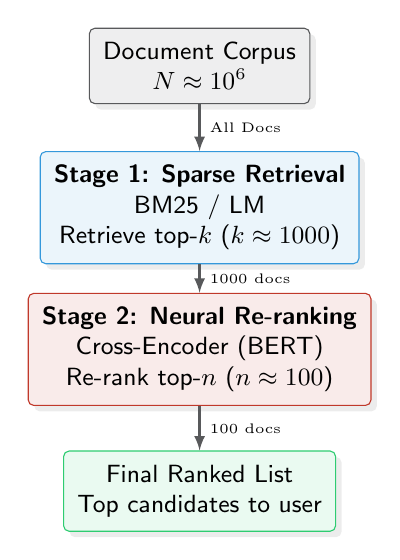
\begin{tikzpicture}[node distance=1.8cm]
    \node[infra] (corpus) {Document Corpus\\$N \approx 10^6$};
    \node[sparse, below of=corpus] (bm25) {\textbf{Stage 1: Sparse Retrieval}\\BM25 / LM\\Retrieve top-$k$ ($k \approx 1000$)};
    \node[rerank, below of=bm25] (rerank) {\textbf{Stage 2: Neural Re-ranking}\\Cross-Encoder (BERT)\\Re-rank top-$n$ ($n \approx 100$)};
    \node[hybrid, below of=rerank] (result) {Final Ranked List\\Top candidates to user};

    \draw[irArrowBase] (corpus) -- (bm25) node[midway, right, font=\tiny] {All Docs};
    \draw[irArrowBase] (bm25) -- (rerank) node[midway, right, font=\tiny] {1000 docs};
    \draw[irArrowBase] (rerank) -- (result) node[midway, right, font=\tiny] {100 docs};
\end{tikzpicture}

\end{center}
\end{frame}

\begin{frame}{Why Two Stages?}
\begin{columns}
\begin{column}{0.48\textwidth}
\textbf{Stage 1: BM25 (Recall-Oriented)}
\begin{itemize}
    \item \textbf{Speed:} microseconds per query
    \item \textbf{Role:} cast a wide net
    \item Catch as many relevant docs as possible
    \item Some irrelevant docs are fine
    \item Metric: \textbf{Recall@1000}
\end{itemize}
\end{column}

\begin{column}{0.48\textwidth}
\textbf{Stage 2: BERT (Precision-Oriented)}
\begin{itemize}
    \item \textbf{Speed:} $\sim$5 ms per doc
    \item \textbf{Role:} sort precisely
    \item Push truly relevant docs to top
    \item Remove false positives from BM25
    \item Metric: \textbf{NDCG@10}
\end{itemize}
\end{column}
\end{columns}

\vspace{1em}

\begin{alertblock}{Critical Dependency}
The re-ranker can only re-order what Stage 1 retrieves. If BM25 misses a relevant document, the cross-encoder can \textbf{never} recover it.

\vspace{0.3em}

\textbf{Recall ceiling from Lecture 2:} Stage 1 determines the ceiling for the entire pipeline.
\end{alertblock}
\end{frame}

\begin{frame}{Pipeline Variants}
\begin{table}
\centering
\small
\begin{tabular}{lccl}
\toprule
\textbf{Pipeline} & \textbf{NDCG@10} & \textbf{Latency} & \textbf{Notes} \\
\midrule
BM25 only & 0.45 & 5 ms & Baseline \\
BM25 + RM3 & 0.49 & 15 ms & Query expansion \\
BM25 + monoBERT & 0.55 & 500 ms & Neural re-rank \\
BM25 + RM3 + monoBERT & \textbf{0.57} & 520 ms & Best sparse+neural \\
BM25 + monoT5-3B & \textbf{0.58} & 2 s & Larger model \\
\bottomrule
\end{tabular}
\end{table}

\small \textit{(Approximate figures on MS MARCO passage ranking)}

\vspace{1em}

\begin{block}{Observations}
\begin{itemize}
    \item Cross-encoder adds $\sim$10 NDCG points over BM25 --- large improvement!
    \item RM3 still helps even with BERT (better Stage 1 recall)
    \item Larger models help but with diminishing returns and higher latency
\end{itemize}
\end{block}
\end{frame}

\begin{frame}{What the Cross-Encoder Fixes}
\textbf{Three categories where BERT improves over BM25:}

\vspace{1em}

\textbf{1. Vocabulary Mismatch}
\begin{itemize}
    \item Query: ``heart attack'' $\to$ BM25 misses ``myocardial infarction''
    \item BERT: cross-attention connects ``heart attack'' to ``myocardial infarction'' {\checkmark}
\end{itemize}

\vspace{0.5em}

\textbf{2. Semantic Relevance vs.\ Topical Overlap}
\begin{itemize}
    \item Query: ``is coffee bad for you'' $\to$ BM25 ranks doc about coffee brands highly
    \item BERT: understands the \textit{health} intent {\checkmark}
\end{itemize}

\vspace{0.5em}

\textbf{3. Negation and Nuance}
\begin{itemize}
    \item Query: ``countries without death penalty'' $\to$ BM25 matches ``death penalty''
    \item BERT: understands ``without'' changes the intent {\checkmark}
\end{itemize}

\vspace{0.5em}

\begin{alertblock}{But Still Fails When\ldots}
BM25 doesn't retrieve the relevant document in top-1000 at all (recall ceiling!).
\end{alertblock}
\end{frame}

% ====================================================================
% SECTION 5: HANDS-ON
% ====================================================================
\section{Hands-On with PyTerrier}

\begin{frame}[plain]
\sectionpage
\end{frame}

\begin{frame}[fragile]{Setup: Loading Index and Models}
\begin{lstlisting}[language=Python]
import pyterrier as pt
if not pt.started():
    pt.init()

dataset = pt.get_dataset('irds:vaswani')
index = pt.IndexFactory.of("./vaswani_index")
topics = dataset.get_topics().head(10)
qrels = dataset.get_qrels()

# BM25 baseline (from Lecture 3)
bm25 = pt.BatchRetrieve(index, wmodel="BM25")

# For neural re-ranking, we use PyTerrier's 
# integration with Hugging Face models
from pyterrier_t5 import MonoT5ReRanker

# Load monoT5 re-ranker (small version for demo)
monoT5 = MonoT5ReRanker(model='castorini/monot5-base-msmarco')
\end{lstlisting}
\end{frame}

\begin{frame}[fragile]{Exercise 1: BM25 vs. Cross-Encoder}
\begin{lstlisting}[language=Python]
# Stage 1: BM25 retrieves top 1000
# Stage 2: monoT5 re-ranks top 100
pipeline_rerank = (bm25 % 100) >> monoT5

# Compare
comparison = pt.Experiment(
    [bm25, pipeline_rerank],
    topics, qrels,
    eval_metrics=["map", "ndcg_cut_10", "P_10"],
    names=["BM25", "BM25 + monoT5"]
)
print(comparison)

# Per-query analysis: which queries improve most?
results_bm25 = pt.Experiment([bm25], topics, qrels,
    eval_metrics=["ndcg_cut_10"], perquery=True)
results_rerank = pt.Experiment([pipeline_rerank], topics, qrels,
    eval_metrics=["ndcg_cut_10"], perquery=True)
\end{lstlisting}
\end{frame}

\begin{frame}[fragile]{Exercise 2: Pipeline Combinations}
\begin{lstlisting}[language=Python]
# Build multiple pipelines
rm3 = pt.rewrite.RM3(index)

pipelines = {
    "BM25": bm25,
    "BM25 + RM3": bm25 >> rm3 >> bm25,
    "BM25 + monoT5": (bm25 % 100) >> monoT5,
    "BM25 + RM3 + monoT5": (
        bm25 >> rm3 >> bm25) % 100 >> monoT5,
}

results = pt.Experiment(
    list(pipelines.values()), topics, qrels,
    eval_metrics=["map", "ndcg_cut_10", "recall_100"],
    names=list(pipelines.keys())
)
print(results)
\end{lstlisting}

\textbf{Discussion:}
\begin{itemize}
    \item Does RM3 still help when BERT re-ranks? (Yes --- better Stage 1 recall)
    \item What is the latency difference?
\end{itemize}
\end{frame}

\begin{frame}[fragile]{Exercise 3: Effect of Re-rank Depth}
\begin{lstlisting}[language=Python]
# How many docs should we re-rank?
depths = [10, 20, 50, 100, 200, 500]
pipelines_depth = {
    f"rerank@{d}": (bm25 % d) >> monoT5
    for d in depths
}

results = pt.Experiment(
    [bm25] + list(pipelines_depth.values()),
    topics, qrels,
    eval_metrics=["ndcg_cut_10", "recall_100"],
    names=["BM25 only"] + list(pipelines_depth.keys())
)
print(results)

# Plot: NDCG@10 vs re-rank depth
# Observe: diminishing returns after ~100
# Also: recall_100 stays same (only reordering!)
\end{lstlisting}

\textbf{Key insight:} Re-ranking deeper costs more time but reaches diminishing returns quickly. The sweet spot is typically 100--200.
\end{frame}

\begin{frame}{Student Exercises}
\begin{block}{Exercise A: Analyze Cross-Encoder Improvements (10 min)}
\begin{itemize}
    \item Find a query where monoT5 significantly improves over BM25
    \item Inspect the top-5 documents from each
    \item Why did BM25 fail? (vocabulary mismatch? topical but not relevant?)
\end{itemize}
\end{block}

\begin{block}{Exercise B: When Does Re-ranking Fail? (10 min)}
\begin{itemize}
    \item Find a query where monoT5 does \textbf{not} help (or hurts)
    \item Check: is the relevant document in BM25's top-1000? (recall ceiling)
    \item What would fix this? (hint: dense retrieval, Lecture 5)
\end{itemize}
\end{block}

\begin{block}{Exercise C: Latency Measurement (5 min)}
\begin{itemize}
    \item Time BM25 alone vs.\ BM25+monoT5 per query
    \item How does re-rank depth affect latency?
    \item What depth gives the best quality-vs-latency trade-off?
\end{itemize}
\end{block}
\end{frame}


% ====================================================================
% SECTION 6: CONNECTIONS
% ====================================================================
\section{Connections and Summary}

\begin{frame}[plain]
\sectionpage
\end{frame}

\begin{frame}{The Representation Spectrum}
\begin{center}
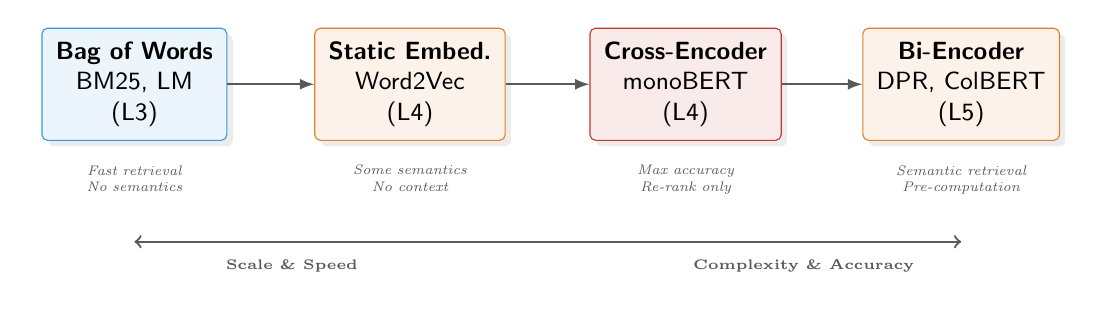
\begin{tikzpicture}
    % Spectrum Nodes
    \node[sparse] (bow) at (0, 0) {\textbf{Bag of Words}\\BM25, LM\\(L3)};
    \node[dense] (static) at (3.5, 0) {\textbf{Static Embed.}\\Word2Vec\\(L4)};
    \node[rerank] (cross) at (7, 0) {\textbf{Cross-Encoder}\\monoBERT\\(L4)};
    \node[dense] (bi) at (10.5, 0) {\textbf{Bi-Encoder}\\DPR, ColBERT\\(L5)};

    % Connections
    \draw[irArrowBase] (bow) -- (static);
    \draw[irArrowBase] (static) -- (cross);
    \draw[irArrowBase] (cross) -- (bi);

    % Captions
    \node[below=0.2cm of bow, irLabel] {Fast retrieval\\No semantics};
    \node[below=0.2cm of static, irLabel] {Some semantics\\No context};
    \node[below=0.2cm of cross, irLabel] {Max accuracy\\Re-rank only};
    \node[below=0.2cm of bi, irLabel] {Semantic retrieval\\Pre-computation};

    % Axis
    \draw[<->, thick, irInfra] (0, -2) -- (10.5, -2);
    \node[font=\tiny\bfseries, irInfra, anchor=north] at (2, -2.1) {Scale \& Speed};
    \node[font=\tiny\bfseries, irInfra, anchor=north] at (8.5, -2.1) {Complexity \& Accuracy};
\end{tikzpicture}

\end{center}

\vspace{0.5em}

\begin{exampleblock}{Today's Key Insight}
Cross-encoders are the \textbf{most accurate} ranking method but \textbf{cannot retrieve}. They must be paired with a fast first stage (BM25 or dense retrieval).
\end{exampleblock}
\end{frame}

\begin{frame}{Cross-Encoder vs.\ Bi-Encoder (Preview of Lecture 5)}
\begin{center}
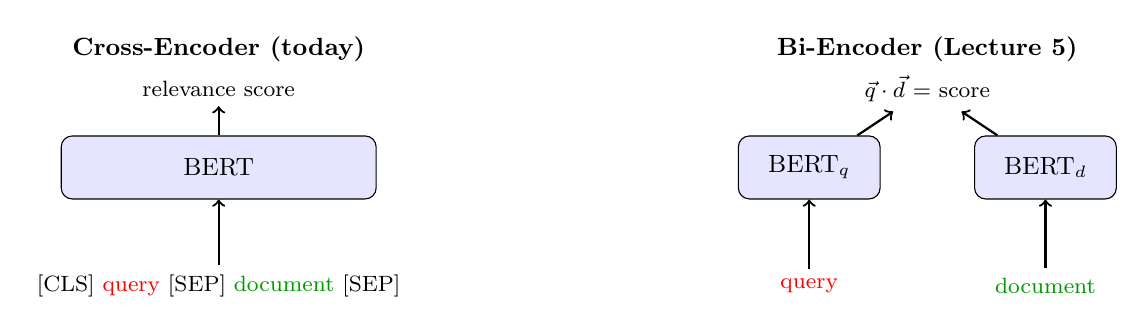
\begin{tikzpicture}[
    box/.style={rectangle, draw, rounded corners, fill=blue!10, minimum height=0.8cm, align=center, font=\small},
    arrow/.style={->, thick}
]
    % Cross-encoder
    \node[font=\small\bfseries] at (-4.5, 3.5) {Cross-Encoder (today)};
    \node[box, minimum width=4cm] (cross_bert) at (-4.5, 2) {BERT};
    \node[font=\footnotesize] (cross_in) at (-4.5, 0.5) {[CLS] \textcolor{red}{query} [SEP] \textcolor{green!60!black}{document} [SEP]};
    \node[font=\footnotesize] (cross_out) at (-4.5, 3) {relevance score};
    \draw[arrow] (cross_in) -- (cross_bert);
    \draw[arrow] (cross_bert) -- (cross_out);

    % Bi-encoder
    \node[font=\small\bfseries] at (4.5, 3.5) {Bi-Encoder (Lecture 5)};
    \node[box, minimum width=1.8cm] (bi_q) at (3, 2) {BERT$_q$};
    \node[box, minimum width=1.8cm] (bi_d) at (6, 2) {BERT$_d$};
    \node[font=\footnotesize, red] (q_in) at (3, 0.5) {query};
    \node[font=\footnotesize, green!60!black] (d_in) at (6, 0.5) {document};
    \node[font=\footnotesize] (dot) at (4.5, 3) {$\vec{q} \cdot \vec{d}$ = score};
    \draw[arrow] (q_in) -- (bi_q);
    \draw[arrow] (d_in) -- (bi_d);
    \draw[arrow] (bi_q) -- (dot);
    \draw[arrow] (bi_d) -- (dot);
\end{tikzpicture}

\end{center}

\vspace{0.5em}

\begin{table}
\centering
\footnotesize
\begin{tabular}{lcc}
\toprule
& \textbf{Cross-Encoder} & \textbf{Bi-Encoder} \\
\midrule
Query-doc interaction & Full (all layers) & None (dot product only) \\
Pre-compute doc embeddings & \textcolor{red}{\ding{55}} No & \textcolor{green}{\checkmark} Yes (offline) \\
Use for retrieval & \textcolor{red}{\ding{55}} No (too slow) & \textcolor{green}{\checkmark} Yes (with ANN) \\
Accuracy & Higher & Lower \\
Speed at inference & Slow & Fast \\
\bottomrule
\end{tabular}
\end{table}
\end{frame}

\begin{frame}{Dual Encoder Architecture}
\begin{center}
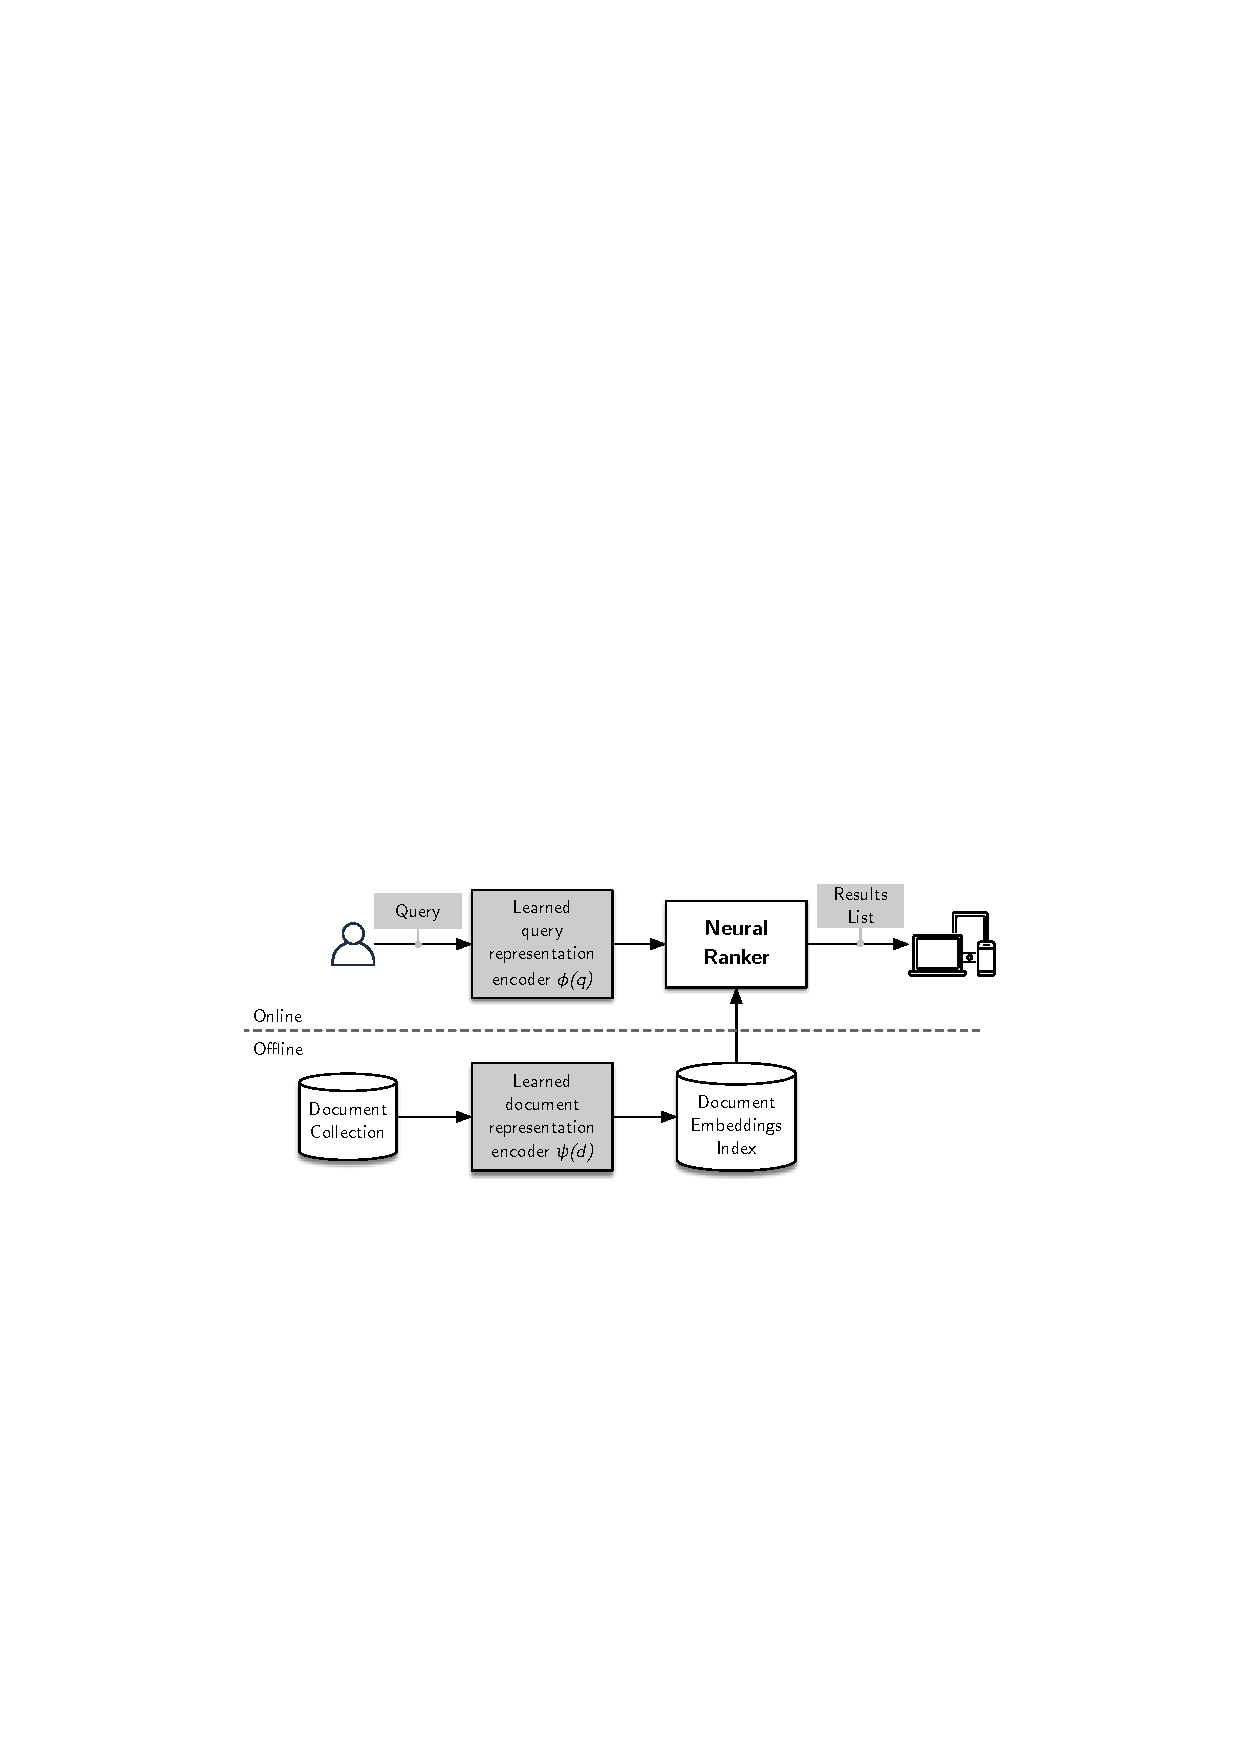
\includegraphics[width=0.85\textwidth]{figures/dual-encoder-ranking.pdf}
\end{center}
\end{frame}


\begin{frame}{Preview: Lecture 5 --- Dense Retrieval}
\begin{block}{The Problem We'll Solve}
Cross-encoders can't retrieve. BM25 misses semantic matches. \\
What if we could do \textbf{semantic retrieval} over the full corpus?
\end{block}

\vspace{0.5em}

\begin{block}{Solution: Bi-Encoders + ANN}
\begin{enumerate}
    \item Encode all documents \textbf{offline} with BERT $\to$ dense vectors
    \item Store in ANN index (IVF+PQ from Lecture 2!)
    \item At query time: encode query with BERT $\to$ ANN search $\to$ top-$k$
\end{enumerate}
\end{block}

\vspace{0.5em}

\begin{exampleblock}{What You'll Learn}
\begin{itemize}
    \item Bi-encoder training: contrastive learning, hard negatives
    \item DPR, ColBERT (late interaction)
    \item Hybrid retrieval: BM25 + Dense
    \item Connection to Lecture 2's ANN indexing (IVF+PQ, FAISS)
\end{itemize}
\end{exampleblock}
\end{frame}

\begin{frame}{Dense Retrieval with ANN}
\begin{center}
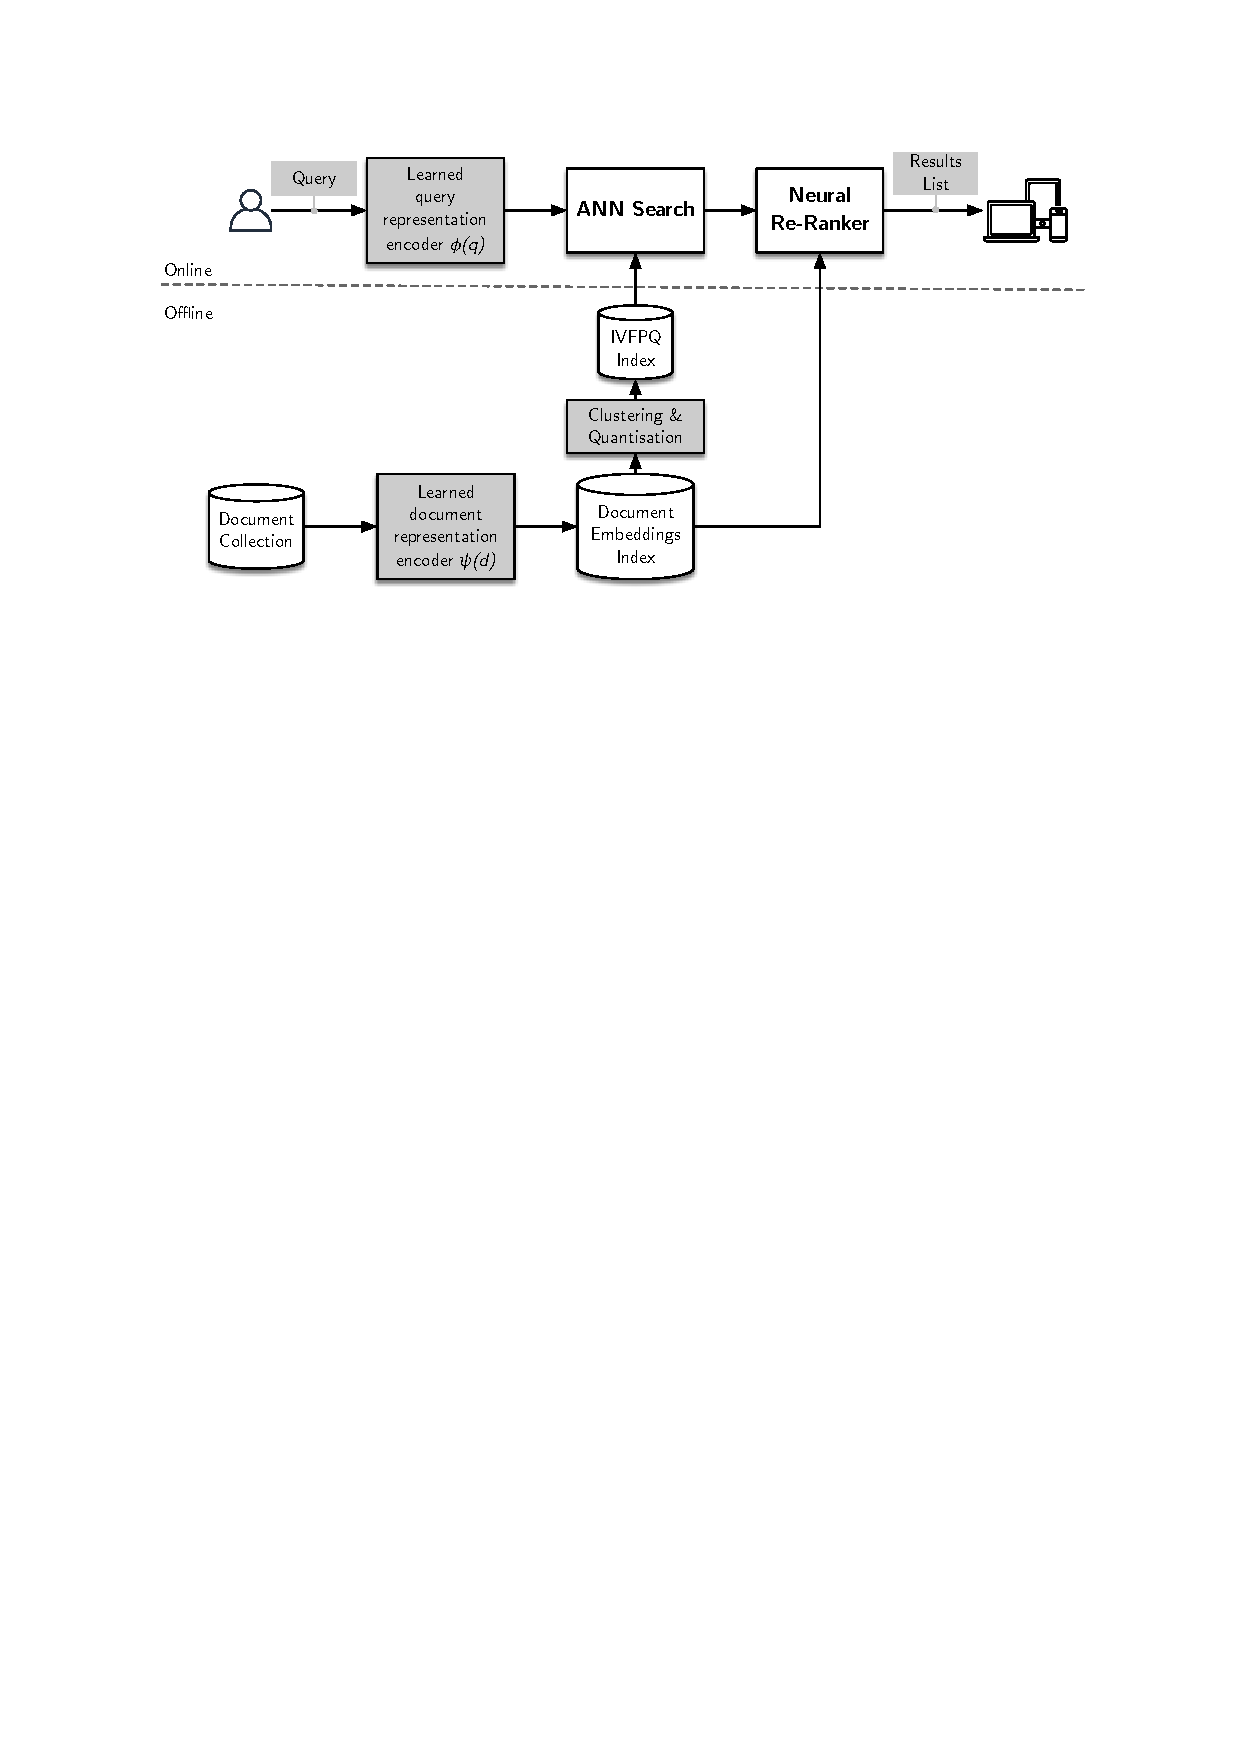
\includegraphics[width=0.85\textwidth]{figures/dense-retrieval-ann.pdf}
\end{center}
\end{frame}


\begin{frame}{Preview: Lecture 6 --- Learning to Rank}
\begin{block}{Connection to Today}
All of today's methods produce \textbf{features} for learning to rank:
\end{block}

\vspace{0.5em}

\begin{itemize}
    \item BM25(q, d) --- sparse relevance score (from Lecture 3)
    \item DirichletLM(q, d) --- language model score (from Lecture 3)
    \item CrossEncoder(q, d) --- BERT relevance score (from today)
    \item DenseScore(q, d) --- bi-encoder similarity (from Lecture 5)
    \item $|d|$, $|q|$, IDF(q), overlap(q, d), \ldots --- metadata features
\end{itemize}

\vspace{0.5em}

\begin{block}{Learning to Rank}
\begin{itemize}
    \item Train a model (LambdaMART) to \textbf{learn the optimal combination}
    \item Directly optimizes ranking metrics (NDCG)
    \item The final piece of the modern retrieval stack
\end{itemize}
\end{block}
\end{frame}

\begin{frame}{The Complete Modern Retrieval Stack}
\begin{center}
\begin{tikzpicture}[node distance=0.8cm]
    \IRBox[10cm]{s1}{(0,0)}{Stage 1: Sparse Retrieval (L3) \textit{or} Dense Retrieval (L5)}{}{sparse}[]
    \IRBox[10cm]{s1b}{(0,0)}{Optional: Query Expansion / PRF improves recall (L3)}{}{hybrid}[below=of s1]
    \IRBox[10cm]{s2}{(0,0)}{Stage 2: Neural Re-ranking / Cross-Encoder}{}{rerank}[below=of s1b]
    \IRBox[10cm]{s3}{(0,0)}{Stage 3: Learning to Rank (LTR) combines all signals (L6)}{Today}{hybrid}[below=of s2]
    \IRBox[10cm]{out}{(0,0)}{Final Ranked List $\to$ User or RAG Application}{}{infra}[below=of s3]

    \IRArrowTB{s1}{s1b}{}
    \IRArrowTB{s1b}{s2}{}
    \IRArrowTB{s2}{s3}{}
    \IRArrowTB{s3}{out}{}
\end{tikzpicture}

\end{center}
\end{frame}

% ====================================================================
% SUMMARY
% ====================================================================
\section{Summary and Assignment}

\begin{frame}[plain]
\sectionpage
\end{frame}

\begin{frame}{Key Takeaways}
\begin{block}{1. Dense Representations Capture Semantics}
Word2Vec/GloVe learn word vectors from co-occurrence. But static embeddings cannot handle polysemy. Contextualized embeddings (BERT) solve this.
\end{block}

\begin{block}{2. Transformers Enable Contextualized Understanding}
Self-attention lets every token attend to every other token. Multi-head attention captures multiple relationship types. Positional encoding preserves word order.
\end{block}

\begin{block}{3. Cross-Encoders Are the Most Accurate Rankers}
BERT cross-encoders process query + document jointly. They understand synonymy, negation, and semantic relevance. But they're too slow for full-corpus retrieval.
\end{block}

\begin{block}{4. The Two-Stage Pipeline Is the Standard Architecture}
BM25 (fast, high recall) $\to$ Cross-encoder (slow, high precision). RM3 can further improve Stage 1 recall. This is how modern search engines work.
\end{block}
\end{frame}

\begin{frame}{Assignment}
\textbf{Continues from Lecture 3 assignment. Additional tasks:}

\vspace{0.5em}

\begin{block}{Part 5: Cross-Encoder Re-ranking (30 pts)}
\begin{itemize}
    \item Add monoT5 re-ranking to your best BM25/RM3 pipeline
    \item Experiment with re-rank depths (20, 50, 100, 200)
    \item Report NDCG@10, MAP, and latency per query
\end{itemize}
\end{block}

\begin{block}{Part 6: Analysis (20 pts)}
\begin{itemize}
    \item Identify 3 queries where cross-encoder helps significantly
    \item Identify 1 query where it fails (recall ceiling)
    \item For each, inspect top-5 docs and explain \textit{why}
    \item Discuss: what would dense retrieval (L5) add?
\end{itemize}
\end{block}

\begin{block}{Deliverable}
Extended Jupyter notebook. Bring your best pipeline to Lecture 5.
\end{block}
\end{frame}

\begin{frame}{Next Class: Dense Retrieval}
\begin{block}{Preparation}
\textbf{Read:}
\begin{itemize}
    \item Karpukhin et al.\ (2020): ``Dense Passage Retrieval for Open-Domain QA''
    \item Khattab \& Zaharia (2020): ``ColBERT: Efficient and Effective Passage Search''
\end{itemize}

\textbf{Skim:}
\begin{itemize}
    \item Reimers \& Gurevych (2019): ``Sentence-BERT''
\end{itemize}
\end{block}

\vspace{0.5em}

\begin{exampleblock}{What We'll Build}
\begin{itemize}
    \item Bi-encoder retrieval over the full corpus
    \item Dense + Sparse hybrid retrieval
    \item Connect to ANN indexing from Lecture 2
    \item The missing piece: semantic matching at retrieval time
\end{itemize}
\end{exampleblock}
\end{frame}

\begin{frame}{Questions?}
\begin{center}
\Huge Questions?

\vspace{2em}

\Large
Office Hours: [Your time]

\vspace{1em}

Email: [Your email]

\vspace{2em}

\normalsize
\textbf{Key formula to remember:}
$$\text{Attention}(Q, K, V) = \text{softmax}\left(\frac{QK^T}{\sqrt{d_k}}\right) V$$
\end{center}
\end{frame}

% ====================================================================
% APPENDIX / BACKUP SLIDES
% ====================================================================
\appendix

\begin{frame}{Backup: BERT Model Sizes}
\begin{table}
\centering
\begin{tabular}{lcccl}
\toprule
\textbf{Model} & \textbf{Layers} & \textbf{Hidden} & \textbf{Params} & \textbf{Use Case} \\
\midrule
BERT-tiny & 2 & 128 & 4M & Debugging \\
BERT-mini & 4 & 256 & 11M & Mobile \\
BERT-small & 4 & 512 & 29M & Lightweight \\
BERT-base & 12 & 768 & 110M & Standard \\
BERT-large & 24 & 1024 & 340M & Best quality \\
\bottomrule
\end{tabular}
\end{table}

\vspace{1em}

\textbf{For IR re-ranking:}
\begin{itemize}
    \item BERT-base is the standard (good quality-to-speed ratio)
    \item BERT-large: $\sim$3$\times$ slower, $\sim$1--2 NDCG points better
    \item DistilBERT: 40\% faster, minimal quality loss (good for production)
\end{itemize}
\end{frame}

\begin{frame}{Backup: Attention Weight Visualization}
\textbf{Query:} ``who founded Tesla'' \quad \textbf{Document:} ``Elon Musk founded Tesla Motors in 2003\ldots''

\vspace{0.5em}

\begin{center}
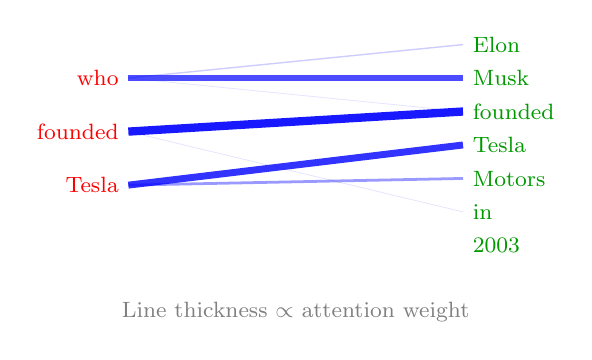
\begin{tikzpicture}[scale=0.85]
    % Query tokens (left)
    \foreach \i/\word in {0/who, 1/founded, 2/Tesla} {
        \node[font=\footnotesize, anchor=east, red] (q\i) at (0, -\i*0.8) {\word};
    }
    % Doc tokens (right)
    \foreach \j/\word in {0/Elon, 1/Musk, 2/founded, 3/Tesla, 4/Motors, 5/in, 6/2003} {
        \node[font=\footnotesize, anchor=west, green!60!black] (d\j) at (5, -\j*0.5 + 0.5) {\word};
    }

    % Attention weights (thicker = higher weight)
    \draw[blue, opacity=0.2, line width=0.5pt] (q0.east) -- (d0.west);
    \draw[blue, opacity=0.7, line width=2pt] (q0.east) -- (d1.west);
    \draw[blue, opacity=0.1, line width=0.3pt] (q0.east) -- (d2.west);

    \draw[blue, opacity=0.9, line width=3pt] (q1.east) -- (d2.west);
    \draw[blue, opacity=0.1, line width=0.3pt] (q1.east) -- (d5.west);

    \draw[blue, opacity=0.8, line width=2.5pt] (q2.east) -- (d3.west);
    \draw[blue, opacity=0.4, line width=1pt] (q2.east) -- (d4.west);

    \node[font=\footnotesize, gray] at (2.5, -3.5) {Line thickness $\propto$ attention weight};
\end{tikzpicture}
\end{center}

\textbf{Observations:}
\begin{itemize}
    \item ``who'' attends strongly to ``Musk'' (answer entity)
    \item ``founded'' attends to ``founded'' (exact match) and weakly to ``in'' (temporal)
    \item ``Tesla'' attends to ``Tesla'' and ``Motors'' (entity span)
\end{itemize}
\end{frame}

\begin{frame}{Backup: Beyond BERT --- Modern Cross-Encoders}
\begin{table}
\centering
\footnotesize
\begin{tabular}{llcl}
\toprule
\textbf{Model} & \textbf{Base} & \textbf{NDCG@10} & \textbf{Key Feature} \\
\midrule
monoBERT & BERT-large & 0.372 & Original, simple \\
monoT5-base & T5-base & 0.364 & Sequence-to-sequence \\
monoT5-3B & T5-3B & 0.384 & Larger $\to$ better \\
RankLLaMA & LLaMA-7B & 0.392 & LLM-based ranking \\
RankGPT & GPT-4 & 0.401 & Listwise re-ranking \\
\bottomrule
\end{tabular}
\end{table}

\small \textit{Approximate TREC DL 2020 figures}

\vspace{0.5em}

\textbf{Trend:} Larger language models make better rankers. But at 7B+ parameters, latency becomes prohibitive for most applications.

\vspace{0.5em}

\begin{block}{RankGPT (Sun et al., 2023)}
Novel approach: give GPT-4 a \textit{list} of documents and ask it to sort by relevance. No fine-tuning needed. Very expensive but very effective.
\end{block}
\end{frame}

\begin{frame}{T5 for Ranking}
\begin{center}
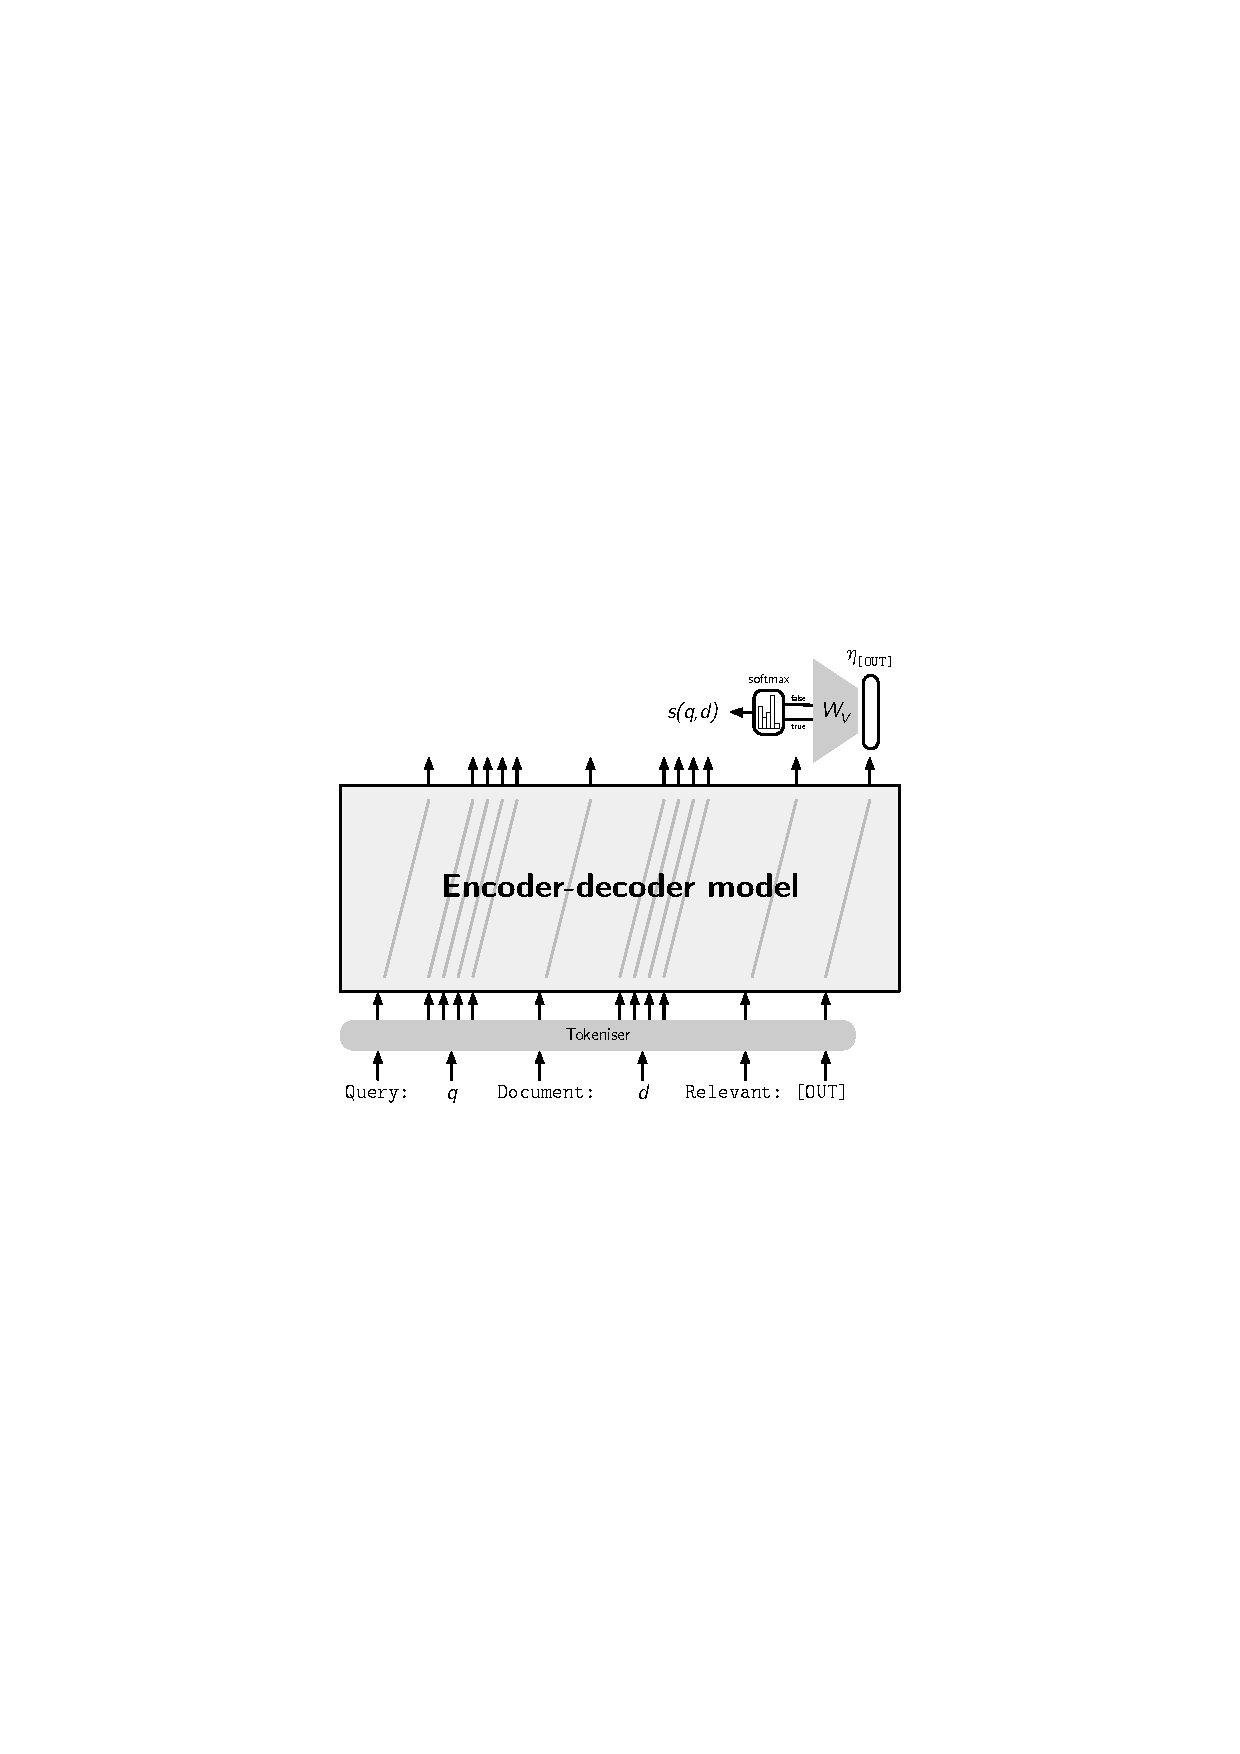
\includegraphics[width=0.8\textwidth]{figures/embeddings-t5-ranking.pdf}
\end{center}
\end{frame}


\begin{frame}{Backup: Tokenization Details}
\textbf{WordPiece Tokenization (BERT):}

\vspace{0.5em}

\begin{table}
\centering
\footnotesize
\begin{tabular}{ll}
\toprule
\textbf{Input} & \textbf{Tokens} \\
\midrule
``information retrieval'' & [``information'', ``retrieval''] \\
``transformers'' & [``transform'', ``\#\#ers''] \\
``subword tokenization'' & [``sub'', ``\#\#word'', ``token'', ``\#\#ization''] \\
``BM25 algorithm'' & [``bm'', ``\#\#25'', ``algorithm''] \\
\bottomrule
\end{tabular}
\end{table}

\vspace{0.5em}

\textbf{Key properties:}
\begin{itemize}
    \item Vocabulary size: 30,522 tokens
    \item Common words: single token (``the'', ``information'')
    \item Rare words: split into subwords (``\#\#'' prefix = continuation)
    \item Max sequence length: 512 tokens (query + document must fit)
    \item \textbf{For IR:} Long documents must be truncated or split into passages
\end{itemize}
\end{frame}

\begin{frame}{Backup: Historical Context}
\begin{center}
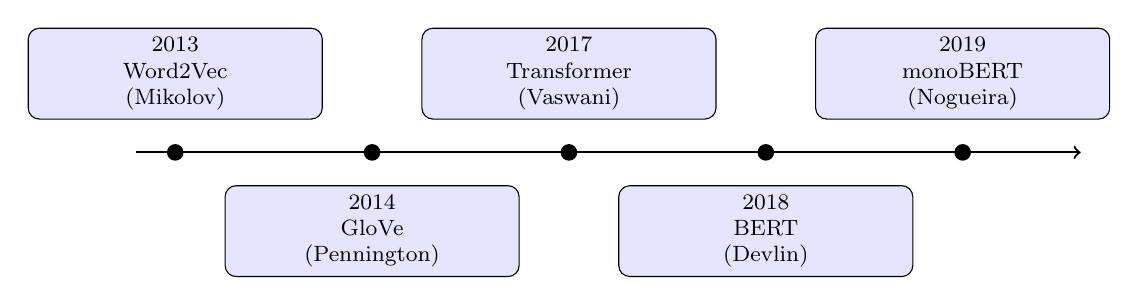
\begin{tikzpicture}[
    event/.style={rectangle, draw, rounded corners, fill=blue!10, text width=3.5cm, align=center, font=\footnotesize, minimum height=0.8cm}
]
    \draw[->, thick] (0, 0) -- (12, 0);

    \node[event] at (0.5, 1) {2013\\Word2Vec\\(Mikolov)};
    \node[event] at (3, -1) {2014\\GloVe\\(Pennington)};
    \node[event] at (5.5, 1) {2017\\Transformer\\(Vaswani)};
    \node[event] at (8, -1) {2018\\BERT\\(Devlin)};
    \node[event] at (10.5, 1) {2019\\monoBERT\\(Nogueira)};

    \foreach \x in {0.5, 3, 5.5, 8, 10.5} {
        \fill (\x, 0) circle (3pt);
    }
\end{tikzpicture}
\end{center}

\vspace{1em}

\textbf{Key milestones for IR:}
\begin{itemize}
    \item 2013: Dense word representations become practical
    \item 2017: Attention mechanism replaces RNNs
    \item 2018: Pre-trained contextual models (transfer learning for NLP)
    \item 2019: First application to IR re-ranking --- large gains over BM25
    \item 2020+: Dense retrieval, hybrid systems, LLM-based ranking
\end{itemize}
\end{frame}

\end{document}